\documentclass[12pt]{report}

\def\magyarOptions{defaults=hu-min}
\usepackage[magyar]{babel}
\usepackage[utf8]{inputenc}
\usepackage{t1enc}

\usepackage{times}

\usepackage{amsmath}
\usepackage{amssymb}
\usepackage{amsthm}

\usepackage{graphicx}
\graphicspath{{figures/}}

\usepackage[bottom,hang,flushmargin]{footmisc}
\usepackage[many]{tcolorbox}

\usepackage{enumitem}
\usepackage{fancyhdr}
\usepackage{float}
\usepackage{hyperref}
\usepackage{makecell}
\usepackage{verbatim}
\usepackage{xcolor}

\usepackage{listings}
\lstset{
    basicstyle=\ttfamily\small,
    rulecolor=\color{gray},
    frame=b,
}

\usepackage{caption}
\DeclareCaptionFont{white}{\color{white}}
\DeclareCaptionFormat{listing}{\colorbox{gray}{\parbox{148mm}{\bfseries#3}}}
\captionsetup[lstlisting]{format=listing,labelfont=white,textfont=white}


% Margins
\hoffset -1in
\voffset -1in
\oddsidemargin 35mm
\textwidth 150mm
\topmargin 15mm
\headheight 10mm
\headsep 5mm
\textheight 237mm

% Colors
\definecolor{qtgreen}{HTML}{44A51C}
\definecolor{qtred}{HTML}{A5441C}

% URL style
\hypersetup{
    colorlinks=false, % Disable colorlinks for not coloring table of contents
    unicode=true,
}

\let\orighref\href
\renewcommand{\href}[2]{%
    \orighref{#1}{\textcolor{blue}{\texttt{#2}}}
}

\let\origurl\url
\renewcommand{\url}[1]{%
    \textcolor{blue}{\origurl{#1}}
}

\newcommand{\todo}[1]{%
    \textcolor{red}{\textbf{TODO:} #1}
}

\newcommand{\fixme}[1]{%
    \textcolor{red}{\textbf{FIXME:} #1}
}

\newcommand{\gerrit}[1]{%
    \textcolor{qtgreen}{\origurl{https://codereview.qt-project.org/\#/c/#1}}
}

\newcommand{\qtbug}[1]{%
    \textcolor{qtred}{\origurl{https://bugreports.qt.io/browse/QTBUG-#1}}
}

\setdescription{
    style=standard,
    align=right,
    itemindent=1cm,
    labelwidth=1cm,
    leftmargin=1cm,
    before={\renewcommand\makelabel[1]{\bfseries ########1:}},
    %font=\sffamily\bfseries,
}

\newtcolorbox{reviewbox}[1][]
  {title=Gerrit Code Review,
   width=12.5cm,
   left=0pt,
   right=0pt,
   fonttitle=\bfseries,
   coltitle=white,
   colframe=qtgreen,
   colback=white,
   #1
}

\newtcolorbox{issuebox}[1][]
  {title=Jira Issue,
   width=12.5cm,
   left=0pt,
   right=0pt,
   fonttitle=\bfseries,
   coltitle=white,
   colframe=qtred,
   colback=white,
   #1
}


\hyphenation{QtWebEngine QtWebKit WebKit Chromium Content Apple Google Quick Widget WebSocket
QtWebSockets QtWebChannel Android WebEngine}

\def\title{A QtWebEngine bővítése és bemutatása saját böngészőalkalmazás segítségével}

\begin{document}

% EMPTY PAGE STYLE
\fancypagestyle{plain}{
    \fancyhf{}
    \fancyfoot[R]{\thepage}
    \renewcommand{\headrulewidth}{0pt}
}

% FOOTER & HEADER
\pagestyle{fancy}
\fancyhf{}
\fancyhead[L]{\title}
\fancyfoot[R]{\thepage}
%\fancyfoot[C]{\thepage}

%%% TITLE PAGE %%%
\thispagestyle{empty}
\begin{center}
    \vspace*{1cm}
    {\Large\textbf{Szegedi Tudományegyetem}}

    \vspace{0.5cm}
    {\Large\textbf{Informatikai Tanszékcsoport}}

    \vspace{3.8cm}
    {\LARGE\textbf{\title}}

    \vspace{3.6cm}
    {\Large Diplomamunka}

    \vspace{4cm}
    \begin{large}
        \begin{tabular}{c@{\hspace{4cm}}c}
            \emph{Készítette:}      & \emph{Témavezető:}        \\
            \textbf{Varga Péter}    & \textbf{Dr. Kiss Ákos}    \\
            programtervező          & egyetemi adjunktus        \\
            informatikus szakos     &                           \\
            hallgató                &
        \end{tabular}
    \end{large}

    \vspace*{2.3cm}
    \begin{Large}
        Szeged

        \vspace{2mm}
        2016
    \end{Large}
\end{center}


%%% TABLE OF CONTENTS %%%
\tableofcontents

%%% PROLOGUE %%%

\chapter*{Feladatkiírás}
\addcontentsline{toc}{section}{Feladatkiírás}

\noindent
A QtWebEngine bővítése úgy, hogy a QtWebKit-et használó fejlesztők könnyen portolhassák
a projektjüket QtWebEngine-re.
Továbbá, olyan új funkciók megvalósítása is fontos, amelyek hozzásegítik a
QtWebEngine-t, hogy lépést tartson a fejlődő web technológiákkal (pl. HTML5).
Az újonnan implementált funkciókat tesztelni kell.

\bigskip
\noindent
A tesztelésre lehetőséget nyújt a Qt \texttt{auto test}
keretrendszere, viszont bizonyos funkciók nem tesztelhetőek megfelelően \texttt{auto}
tesztekkel, továbbá nem biztosítható teljes lefedettség. A probléma kiküszöbölésére
példa alkalmazás(ok) implementálására van szükség, amelyet a fejlesztő használhat
``manuális'' tesztelésre, hibakeresésre, továbbá annak forráskódja a funkciók
dokumentálására, bemutatására is felhasználható.

\bigskip
\noindent
A fejlesztés során az alábbi szempontokat kell figyelembe venni:
\begin{itemize}
    \item Bináris kompatibilitás megtartása korábbi QtWebEngine verziókkal:
        publikus API-ban a változtatások számát minimalizálni kell,
        meglévő API-t (függvény, property, signal, stb.) módosítani vagy eltávolítani
        nem lehet.
    \item Törekvés kompatibilitásra a QtWebKit-el.
        A QtWebEngine-hez adott új API-k ne térjenek el (névben, paraméterezésben, stb.)
        az eredeti QtWebKit API-tól, hacsak ezt az új funkcionalitás bővítése nem indokolja.
    \item Törekedni kell arra, hogy a Quick és Widget API hasonlítson egymásra,
        amennyire csak lehet.
    \item Az új funkcionalitásokhoz \texttt{auto} tesztet kell készíteni,
        ahol ez megoldható.
    \item Qt 5.6-os verziójától minden új funkcionalitást dokumentálni kell.
\end{itemize}


\chapter*{Tartalmi összefoglaló}
\addcontentsline{toc}{section}{Tartalmi összefoglaló}
\begin{itemize}
    \item \textbf{A téma megnevezése:} \\
        \title
    \item \textbf{A megadott feladat megfogalmazása:} \\
        A QtWebEngine bővítése új funkciókkal és azok tesztelése a
        Qt teszt keretrendszerének segítségével. Az új funkciók bemutatása
        egy saját böngészőalkalmazás megvalósításával.
    \item \textbf{A megoldási mód:} \\
        Részvétel a QtWebEngine project fejlesztésében. Az új funkciók
        megvalósítása \texttt{C++} nyelven. Egy példa böngészőalkalmazás implementálása
        QtQuick használatával, \texttt{C++} és \texttt{QML} nyelven.
    \item \textbf{Alkalmazott eszközök, módszerek:} \\
        A fejlesztés GNU/Linux rendszeren, QtCreator fejlesztői
        környezetben (IDE) történt. A hibakereséshez GDB-t használtam.
        Makefile-ok legenerálását a project file-okból a qmake végzi.
        A project fordítása Linux-on a GNU Toolchain-el (GCC 5.3),
        Os X-en Xcode-al (Xcode 7.2.1), Windows-on pedig
        MSVC 2013 32-bites verziójával történt. A verzió-követéshez Git-et
        használtam. A teszteléshez szükséges keretrendszert és a teszteket a Qt
        repository-k tartalmazzák.
    \item \textbf{Elért eredmények:} \\
        A QtWebEngine 8 új funkcióval lett kibővítve. Ebből 4 a QtWebKit-ből
        átvett, 3 a tesztelést és hibakeresést segíti, 1 pedig HTML5 funkció.
    \item \textbf{Kulcsszavak:} \\
        \texttt{QtWebEngine}, \texttt{QtWebKit}, \texttt{QtQuick}, \texttt{Qt},
        \texttt{Chromium}, \\
        \texttt{Chromium Content API}, \texttt{Web}, \texttt{HTML5}, \texttt{WebKit},
        \texttt{Blink}, \texttt{C++}, \texttt{QML},\\
        \texttt{Quick}, \texttt{Widget}, \texttt{WebEngineView}
\end{itemize}

%%% CONTENT %%%

\chapter*{Bevezetés}
\addcontentsline{toc}{section}{Bevezetés}
A QtWebEngine-t 2013-ban kezdték el fejleszteni a Qt fejlesztői kísérleti jelleggel
a WebKit--Chromium szétválás után. A szétválás előtt a Qt fejlesztői csapata volt a harmadik
legtermékenyebb contributor-a (hozzájárulója) a WebKit kód bázisnak, az Apple és a
Google után. A kérdés adott volt: megtartsa e a Qt jól bevált QtWebKit komponensét és
maradjon az Apple szárnysegédje, vagy beálljon az új lehetőségeket és irányt mutató Google
mögé azáltal, hogy az ő web platformjára épít egy új API-t. Végül az utóbbi mellett
döntöttek, a QtWebKit projektet parkolópályára helyezték és a QtWebEngine éles lett.
\cite{bib:qt-blog-introducing-qtwebengine}

2014 elején kapcsolódtam be a projektbe és azóta is részmunkaidőben veszek részt a
fejlesztésekben. Az azóta eltelt több, mint 2 év alatt sokat tanultam a Qt-ról,
Chromium-ról és a web technológiákról, úgy egyáltalán. Dolgozatomban az ez idő alatt
gyűjtött tapasztalatokból szeretnék megörökíteni egy szeletet.

A QtWebEngine (korábban QtWebKit) projekt célja egy Qt modul (függvénykönyvtár) nyújtása a
fejlesztők számára, amelynek használatával könnyedén integrálhatnak böngésző
funkcionalitásokat saját Qt alkalmazásaikba vagy könnyedén valósíthatnak meg Qt platform
felett saját böngészőt. Ráadásul, mindezt úgy tehetik meg, hogy nincs szükségük semmilyen
ismeretre arról, hogy egy böngésző, hogyan működik a motorháztető alatt.

Dolgozatomat 3 részre tagoltam. Az első részben adok áttekintést arról, hogy mi is az a
Chromium, mi a Qt, ezek hogyan kapcsolódnak egymáshoz és hogyan is lesz ebből QtWebEngine.
A második részben összegyűjtöttem 8 olyan funkcionalitást (feature-t), amit magam
fejlesztettem és adtam hozzá a QtWebEngine-hez. Röviden leírom, hogyan valósítottam meg
őket, mi volt a célom velük és milyen nehézségekkel kellett szembe néznem a megvalósítás
során.

A legutolsó fejezetben szeretném bebizonyítani, hogy könnyű a QtWebEngine-el böngészőt
készíteni. Sajnos a Chromium erőforrás igénye és a magas szintű API-ja miatt, nem várható el
a QtWebEngine-től, hogy lekörözze sebességben és/vagy memória-fogyasztásban a versenytársakat.
A QtWebEngine igazi előnye kétség nélkül az egyszerű használhatóságban és a cross-platform
támogatásban rejlik.


\chapter{Áttekintés: \mbox{Chromium + Qt = QtWebEngine}}

\section{Chromium}
A Chromium a Google által fejlesztett, nyílt forrású (open source) web böngésző projekt. Nagy
része \texttt{C++} nyelven íródott. Támogatja napjaink legnépszerűbb operációs rendszereit \\
(``cross-platform''), legyen az desktop (Windows, Linux, OS X) vagy mobil (Android, iOS,
QNX).
A Chromium nem egy böngésző alkalmazás, hanem egy tabokat használó ablakkezelő (vagy shell)
a web-hez.
\cite{bib:wiki-chromium}

\subsection{Chrome}
A Google saját Chromium-ra épülő böngésző alkalmazása a Google Chrome.
Ez az alkalmazás Chromium-mal szemben nem nyílt forrású, viszont a böngésző
megvalósításának nagy része a Chromium projektben megtalálható.
A Chrome nem nyílt részei például a beépített Adobe Flash Player (Pepper Flash Player)
és az automatikus frissítésekért felelős komponens (GoogleUpdate). \cite{bib:wiki-chrome}
Egy másik, szintén népszerű Chromium-ra épülő böngésző alkalmazás az Opera.

\subsection{Blink}
A Chromium 28-as verziójától kezdve a Blink böngésző motort használja.
A böngésző motor elsődleges feladata a webes tartalom megjelenítése a képernyőn. Talán
ebből is látszik, hogy a Blink talán a legfontosabb komponense a Chromium-nak.
A Chromium a 28-es verzió előtt WebKit-et használt, a Google ezt a projektet forkolta és
nevezte el Blink-nek. Pontosabban, annak csak egy részét, név szerint a WebCore-t.
\cite{bib:wiki-blink}

A Blink nem tartalmazza a WebKit-ben alkalmazott multi-processz architektúrát és sandbox
megoldást, ezek a feladatok a Chromium más szintjein vannak megvalósítva, így egyszerűbbé
téve a Blink forráskódját.
Továbbá, a WebKit része JavaScriptCore JavaScript motor is, ami a Blink-be már nem került
bele, hiszen a Chromium-nak van sajátja, a V8. Ezektől eltekintve a Blink még mindig nagyon
hasonlít a WebCore-ra/WebKit-re. A Chromium forrásában és könyvtár struktúrájában továbbra is
``WebKit'' néven hivatkoznak erre a komponensre\footnote{Például, a Blink forrása a
\texttt{third\_party/WebKit} könyvtárban található a Chromium repository-n belül}.
\cite{bib:chromium-displays-web-pages, bib:chromium-blink}

A Blink az a komponens, ami a weboldal tartalmát feldolgozza és előkészíti megjelenítésre.
Az oldal tartalmát először parse-olja és a HTML elemekből \texttt{Node} objektumokat gyárt.
Ezeket a \texttt{Node}-okat egy fába rendezi, amit DOM (Document Object Model) fának hívnak.
A DOM fának a gyökér \texttt{Node}-ja mindig, az úgynevezett, \texttt{Document Node}.
A fa építése során, a motor, minden megjeleníthető \texttt{Node}-hoz egy
\texttt{RenderObject}-et rendel. A \texttt{RenderObject} az az elem, ami ``tudja'',
hogyan kell a hozzátartozó \texttt{Node}-ot megjeleníteni.
A DOM fa építésével párhuzamosan, a Blink egy másik fát is épít a
\texttt{RenderObject}-ekből, ez a \texttt{Render Tree}. Továbbá, bizonyos
\texttt{RenderObject}-hez \texttt{RenderLayer}-t is rendel, amiből egy újabb fát épít,
ami pedig a \texttt{RenderLayer Tree}.

\begin{figure}[h]
    \centering
    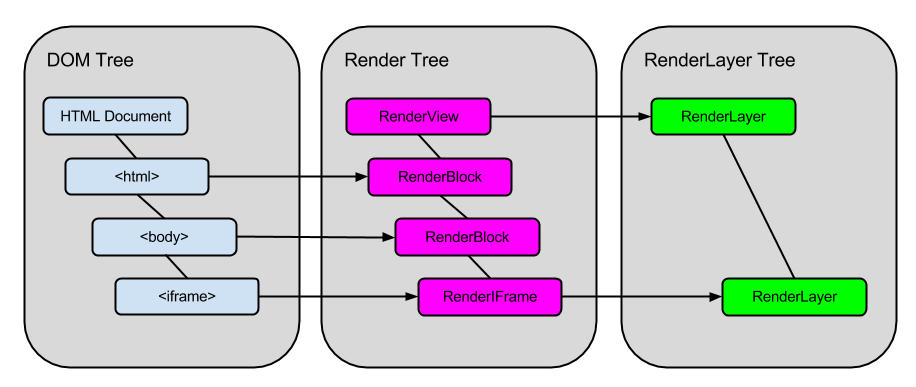
\includegraphics[scale=0.46]{rendering-trees}
    \caption{
        \label{fig:rendering-trees}
        Rendering Trees \cite{bib:chromium-oopifs}
    }
\end{figure}

\noindent
Az \ref{fig:rendering-trees} ábra szemlélteti, hogyan is állnak össze ezek a struktúrák.
A \texttt{DOM Tree} és a \texttt{Render Tree} szinte azonos, annyi különbséggel, hogy
a \texttt{Render Tree} csak a megjeleníthető \texttt{Node}-okat tartalmazza.
A \texttt{RenderLayer Tree} a \texttt{Render Tree} egy lecsupaszított változata, amit a
megjelenítő komponens (renderer) fog használni a rajzoláshoz.
A \texttt{RenderLayer}-ből elérhetőek a \texttt{RenderObject}-ek, a \texttt{RenderLayer Tree}
szerkezete pedig, hordozza azt az információt, hogy milyen sorrendben kell kirajzolni
\texttt{RenderObject}-eket és, hogy azok között milyen átfedések lehetnek.

Az, hogy a rajzolás hogyan történik az függ attól, hogy van e elérhető hardveres gyorsítás.
Ha nincs, akkor szoftveres renderelés történik. A szoftveres renderelés során a rajzoló
algoritmus bejárja a \texttt{RenderLayer Tree}-n keresztül a \texttt{RenderObject}-eket és
azokat egy közös bitmap-re rajzoltatja ki. Ha kész, ez a bitmap lesz elküldve egy másik
processz (browser process) számára megjelenítésre. Szoftveres renderelés esetén a rajzolást
a Skia grafikus motor végzi.

Ha van elérhető hardveres gyorsítás, akkor az eljárás valamivel bonyolultabb. Ebben az
esetben, a \texttt{RenderObject} nem bitmap-be ``rajzolja bele magát'', hanem 3D API-n
keresztül (OpenGL vagy Windows-on esetleg D3D) utasításokat küld közvetlenül a GPU
utasítás pufferébe (command buffer) végrehajtásra. Ezt az eljárást már a
Chrome Compositor (CC) végzi.
\cite{bib:chromium-gpu, bib:chromium-oopifs}

\subsection{Chrome Compositor (CC)}
A Chrome Compositor már nem része a Blink-nek (ahogy a Skia sem). Ennek az az oka,
hogy most már a Chromium a browser UI megrajzolásához is a Chrome Compositor-t használja.
Ahhoz, hogy a compositor ki tudja rajzolni a DOM-ban tárolt tartalmat, további layer
absztrakciókra van szükség:
\begin{center}
    \texttt{RenderLayers} $\rightarrow$ \texttt{GraphicsLayers} $\rightarrow$
    \texttt{WebLayers} $\rightarrow$ \texttt{CC Layers}
\end{center}

A compositor a végeredményt nem bitmap-be, hanem textúrába ``rajzolja''. Az elkészült
textúrák a GPU memóriájában vannak tárolva és úgy nevezett texture mailbox segítségével
azonosítják. A texture mailbox egy OpenGL extension kiterjesztés, ami egyedi és globális
string azonosítót rendel a textúrához és lehetővé teszi, hogy más OpenGL context-en
is elérhető legyen a textúra, ami normális esetben nem lenne megosztva.
\cite{bib:chromium-gpu, bib:chromium-oopifs}

A texture mailbox-nak hála az összeállított képet nem kell az IPC-n (Inter-Process
Communication) keresztül megosztani a processzek között (mint a szoftveres rendering
esetében), hanem a GPU memórián keresztül bármelyik processz hozzáférhet a textúrához, így
elég csak a textúra azonosítót átküldeni IPC-n.
\cite{bib:chromium-texture-mailbox}

\subsection{Multi-processz Architektúra}
Chromium volt az egyik első olyan böngésző, ami úgy lett megtervezve, hogy több processzre
legyen felosztva. A WebKit multi-processz architektúrára épülő API-ja (WebKit2) is a
Chromium-ról vette a mintát. \cite{bib:webkit-webkit2}
Ez az API a Blink-nek nem része, viszont a QtWebEngine elődjének, a QtWebKit-nek
Quick API-ja a WebKit2-re épül.

A multi-processz architektúrán alapuló böngésző alapgondolata az, hogy a böngészőalkalmazás
UI-ért felelős része saját processzben fut, míg a weboldalak megjelenítésért más
processzek felelnek. Ennek több előnye is van: \cite{bib:chromium-blog-multi-process}
\begin{description}
    \item[Felhasználói élmény]
        Előfordulhat, hogy egy weboldalon futó script (vagy ``webalkalmazás'')
        nagyon leterheli a böngészőt. Ha ez a script és a UI egy processzben fut,
        akkor ezek nagyobb valószínűséggel vonnak el egymástól erőforrást. Ha külön
        processzben, egymástól függetlenül futnak, kisebb valószínűséggel alakul ki
        köztük versenyhelyzet, így a UI nagyobb CPU használatnál is ``reszponzívabb''
        lehet.
    \item[Biztonság]
        Egyes processzek sandbox-ban futhatnak. Ezáltal nem férhetnek hozzá a rendszer
        olyan erőforrásaihoz, ami veszélyes lehet (pl. merevlemez, hálózat,
        videó memória, stb).
        Továbbá a különböző weboldalakat megjelenítő processzek egymástól is el vannak
        különítve, így egy ártalmas oldal, vagy plugin nem férhet hozzá más oldalon használt
        szenzitív információhoz (pl. jelszó).
    \item[Hibatűrés, Robosztusság]
        Ha egy oldal betöltésekor vagy egy bővítmény futtatásakor hiba történik és
        összeomlik, az nem rántja magával a teljes böngészőt. Hiba esetén a UI és más
        megnyitott oldalak, tabok megmaradnak.
\end{description}

A multi-processz architektúrának hátrányai is vannak: ez a megoldás sokkal \\
erőforrás-igényesebb, és a megvalósítás is bonyolultabb (több hibalehetőség).
A processzek használata memória többletköltséggel jár. Továbbá, a futtatható processzek
számát limitálni kell, mert túl sok processz jelentős lassulást okozhat (pl. az ütemező
többletköltsége miatt).

A processzek IPC-n (Chromium's IPC System) keresztül kommunikálnak egymással.
A Chromium-ban 4 fő processz típust különböztetünk meg:

\subsubsection{Browser Process}
Ez az a processz, ahol maga böngésző alkalmazás (UI) fut. Ez felelős megjelenítésért,
a felhasználói események és a tabok kezeléséért. Ez a fő processz, ami a többi processzt
kezeli (indítja, leállítja, stb.) és csak egy van belőle. Hozzáfér a rendszer erőforrásaihoz,
viszont nem tölt be vagy dolgoz fel web tartalmat.

\subsubsection{Render Process}
A renderelő motor egy nagyon összetett és bonyolult szoftver komponens. Szinte lehetetlen
olyat implementálni, ami sosem hibázik és/vagy omlik össze. \cite{bib:chromium-multi-process}
Ezért racionális döntés az egymástól független oldalak renderelését egymástól független
processzekben végrehajtani. Amennyiben egy Render Process összeomlik, arról a
Browser Process értesül és az oldal helyett az \ref{fig:sad-tab} ábrán látható,
úgynevezett, ``sad tab'' értesítést jeleníti meg.

\begin{figure}[h]
    \centering
    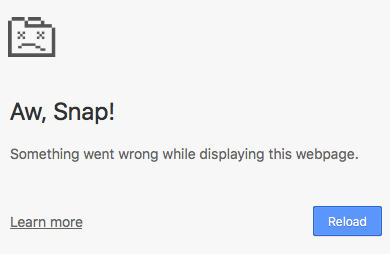
\includegraphics[scale=0.8]{sad-tab}
    \caption{
        \label{fig:sad-tab}
        Sad Tab
    }
\end{figure}

Mivel a Chromium-ban a renderelésért a Blink felel, ezért az is a Render Process-ben fut.
A Blink az, ami közvetlenül feldolgozza a webes tartalmat, ezért jellemzően a
Render Process-t sandbox-ban futtatják, így a potenciálisan kártékony webes kódok nem
férhetnek hozzá a rendszer erőforrásaihoz vagy más betöltött webes tartalomhoz.

A Chromium-ban különböző parancssori kapcsolókkal is beállítható processz modellek
vannak definiálva:
\begin{description}
    \item[Process-per-site-instance]
        Minden site\footnote{Site alatt olyan weboldalak csoportját értjük, amelyek
        közös beregisztrált domain néven osztoznak} külön processz.
        Ha ugyanaz a site kétszer van megnyitva, akkor az is két külön processz lesz.
    \item[Process-per-site]
        Különböző site-ok külön processzbe kerülnek. Az előzővel ellentétben, ha egy site
        kétszer van megnyitva, akkor azok közös processzbe kerülnek.
    \item[Process-per-tab]
        Minden tab külön processz. Több tab kerülhet közös processzbe, ha függnek egymástól.
    \item[Single Process]
        A ``hagyományos, egy-processzes'' modell. \\
        Nincs külön Render Process. A rendering a Browser Process-ben történik.
\end{description}

\noindent
Alapértelmezetten a \textit{Process-per-site-instance} modellt használja a böngésző, de
ettől függetlenül előfordulhat, hogy több site is osztozik, ugyanazon a processzen.
Erre vagy akkor van szükség amikor két site hivatkozik script-ből egymásra,
vagy amikor a futó Render Proess-ek száma elér egy limitet.
\cite{bib:chromium-process-models}

\subsubsection{Plugin Process}
A pluginok okozzák a legtöbb problémát a böngésző stabilitásának szempontjából. A plugint
egy harmadik fél készíti ezért a Chromium-nak nincs befolyása afelett, hogy milyen
erőforrásokat használ. Ennél fogva, indokolt lépés a pluginokat nem a Browser Process-ben
futtatni. A legtöbb plugin nem futhat sandbox-ban, mivel olyan
képességekkel bővítik a böngészőt, amelyekhez szükség van hozzáférésre a rendszer
erőforrásaihoz. Ezért a Render Process-en kívül szükség van egy újabb processz típusra is,
amelyben a pluginok futhatnak.
\cite{bib:chromium-plugins}

\subsubsection{GPU Process}
A renderelés a Render Process-ben történik, viszont ez a processz sandbox-ban fut és ezért
nem küldhet parancsokat GPU-nak. Hardveres gyorsítás esetén a compositing-ot és a rajzolást
egy külön processzben kell végezni, ami nem sandbox-ban fut.
\cite{bib:chromium-gpu} \\
A Chromium úgy is konfigurálható, hogy a GPU Process feladatát a Browser Process lássa el.

\subsection{Chromium Content Module}
A Content Module a Chromium az a része, ami megvalósítja az előző fejezetben bemutatott
multi-processz architektúrát. Továbbá, ebben van megvalósítva az összes támogatott
web platform funkcionalitás (például: HTML5, WebRTC, WebGL, stb.), illetve
a hardveres GPU gyorsítás. Böngészőalkalmazás specifikus funkcionalitások, nem részei
Content Module-nak. Lényegében csak az van benne, ami a web tartalom
megjelenítéséhez\footnote{\textit{content} = web tartalom} szükséges, azaz olyan kód,
amit minden böngészőt integráló alkalmazásnak szüksége van.
\cite{bib:chromium-content-module}

A modul célja, hogy az opcionális böngésző funkcionalitások (amire nem feltétlenül van
szüksége a beágyazó alkalmazásnak (pl. Chrome) le legyenek választva, ezáltal
megvalósíthatóak és testreszabhatóak legyenek a beágyazó alkalmazásban anélkül,
hogy a Chromium forráskódját módosítani kellene. Erre nyújt lehetőséget a Content API.

\subsubsection{Chromium Content API}
A Content API megtervezésekor a WebKit API-t vették alapul, hogy a WebKit fejlesztők
könnyebben áttérhessenek. Az új API \textit{unstable}, ami azt jelenti, hogy az API minden
új kiadásban változhat, ezért a beágyazó alkalmazást is minden Chromium frissítés után nagy
valószínűséggel változtatni kell.

A Content Module a beágyazó alkalmazást interfészeken (Delegate, Observer)
és callback függvényeken keresztül értesíti az eseményekről, változásokról (például,
hol tart a web oldal letöltése vagy sikeres volt-e a letöltés) vagy éppen
kér le adatokat (például, kell megjeleníteni hiba üzenetet, ha nem sikerül letölteni egy
oldalt). Az ilyen interfészek metódusainak törzse üres a Content Module-ban, ezeket a
beágyazó alkalmazásnak kell megvalósítania és a Content Module hívja meg őket szükség esetén.

Ezeken kívül vannak olyan interfészek is, amelyeket a Content Module implementál
(például, oldal betöltése: \texttt{LoadURLWithParams()} vagy az URL lekérdezése: \\
\texttt{GetVisibleURL()}).
Ezek az interfészek \textit{pure abstract} interfészek, mivel csak egy megvalósításuk lehet
és az is a Content Module-on belül. \cite{bib:chromium-content-api}

\subsubsection{Chromium Content Shell}
\begin{figure}[h]
    \centering
    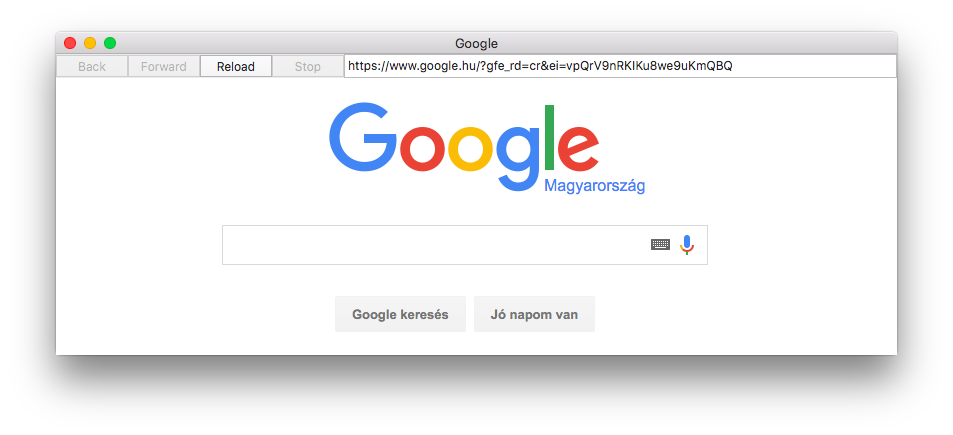
\includegraphics[scale=0.5]{content-shell}
    \caption{
        \label{fig:content-shell}
        Content Shell
    }
\end{figure}

\noindent
Az \ref{fig:content-shell} ábrán látható alkalmazás a Content Shell. Ez a lehető
legegyszerűbb böngészőalkalmazás, ami a Content API-ra épül. Arra használják, hogy a
Content Module-t és a Blink-et tesztelhessék, debuggolhassák anélkül, hogy egy teljes
böngészőalkalmazást (pl. Chrome) le kellene fordítani.

\subsection{Felépítés}
Az eddigiek alapján a Chromium-ot 3 rétegre oszthatjuk fel:
\begin{description}
    \item[Chrome]
        Felhasználói felület (UI) és böngészőalkalmazás funkciók
        (pl.: history, könyvjelzők, favicon, stb.)
    \item[Blink]
        Webes tartalom feldolgozása és renderelése. A V8 JavaScript motort a
        Blink-en keresztül érjük el és közös processzben futnak.
    \item[Content]
        Ez a réteg valósítja meg a multi-processz architektúrát,
        felel a web platform funkciókért és a hardveres GPU gyorsításért.
\end{description}
A \ref{fig:chromium-architecture} ábra mutatja, hogyan is állnak össze a Chromium rétegei.
Itt a Blink böngészőmotor még ``WebKit''-nek van jelölve.
A legfelső réteg a Chrome, helyére a saját beépítő alkalmazás kerül.

\begin{figure}[h]
    \centering
    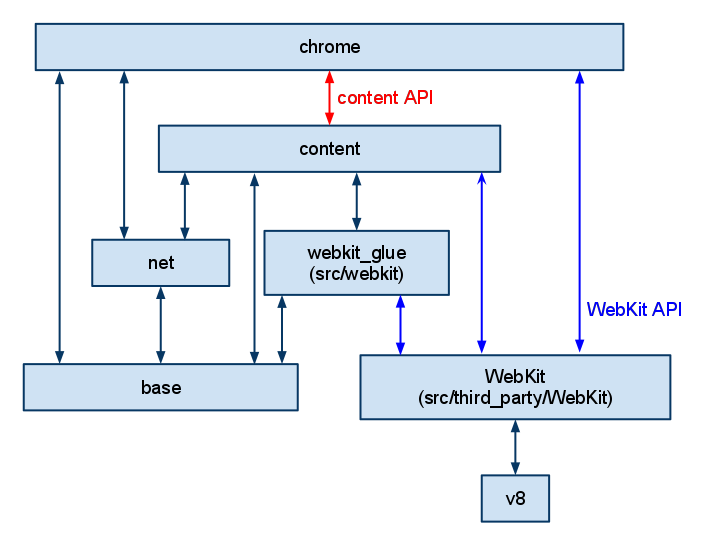
\includegraphics[scale=0.6]{chromium-architecture}
    \caption{
        \label{fig:chromium-architecture}
        Chromium Architecture \cite{bib:chromium-content-module}
    }
\end{figure}


\subsection{Release}
Egy Chromium release verzió száma 4 részből tevődik össze:
\begin{verbatim}
    MAJOR.MINOR.BUILD.PATCH
\end{verbatim}
A dolgozatomban a főverzió számra (\texttt{MAJOR}) hivatkozok.
A Chromium közösség előre tervezett menetrend szerint 1-1.5 havonta vált főverzió számot
(ad ki új release-t).
Dolgozatom készítése idején az 51-es verziójú volt a legfrissebb stabil kiadás.
Az itt leírtak erre a verzióra vonatkoznak.


\section{Qt}
A Qt egy nyílt forrású, cross-platform alkalmazás keretrendszer. Úgy ahogy a
Chromium úgy a Qt is elérhető napjaink legnépszerűbb desktop és mobil
operációs rendszerein. Ez a keretrendszer nyújt \texttt{C++} függvénykönyvtárakat (library),
binding-okat más programozási nyelvekhez (pl.: Python, Java), saját programozási nyelvet
(\texttt{QML}), saját integrált fejlesztői környezetet (QtCreator), saját build rendszert
(qmake) és kiterjesztéseket is a \texttt{C++} programozási nyelvhez (pl.: signal-slot model).
\cite{bib:qt-wiki-about-qt}

\subsection{Történelem}
\subsubsection{1995-2000}
A Qt első verziója 1995-ben adta ki a Trolltech. Akkor még a projekt egy
cross-platform GUI fejlesztői keretrendszernek indult.
Nem sokkal később (1998-ban), jelent meg a
KDE (K Desktop Environment) első verziója, amely Qt-re épült.
A KDE egyhamar az egyik legnépszerűbb Linuxos asztali környezetté nőtte ki magát
és talán ennek tudható be a Qt népszerűsége is.
A Qt eszköztára az évek során fokozatosan
bővült. Új API-k jelentek meg adatbázis kezeléshez (SQL), hálózati programozáshoz,
multimédiás alkalmazások készítéséhez, XML dokumentumok feldolgozásához stb.

\subsubsection{2000-2008}
2000-ben megjelent a Qt-ra épülő Qt/Embedded keretrendszer Linux-os beágyazott eszközökre.
Ezzel az új technológiával a Qt meg is jelent az első okos telefonokon (2003: Motorola A760)
és a korabeli PDA-kon. 2006-ban a Trolltech még a saját fejlesztésű mobil telefonját is
kiadta, Greenphone néven.

\subsubsection{2008-2011}
Talán a Trolltech beágyazott platformokon és mobil telefonokon szerzett tapasztalata
miatt került arra sor, hogy 2008-ban, az akkori egyik vezető mobiltelefon gyártó, a Nokia,
felvásárolta a céget. A következő pár évben a fejlesztés még inkább a mobil eszközök
felé irányult, olyannyira, hogy azokon a részeken, melyek nem voltak érintettek mobil
fejlesztés szempontjából jóformán nem is történt fejlesztés.
2010-ben kiadott 4.7-es verzióban két nagyon fontos újítás (teljesen új modul) jelent meg:
a QtWebKit és a QtQuick.

A WebKit az Apple által fejlesztett nyílt forrású böngésző motor, a QtWebKit pedig ennek
a ``Qt portja''. Ez azt jelenti, hogy az API természetesen ``Qt-s'', továbbá a legfontosabb
``alacsony szintű'' feladatokat is a Qt látja el, mint például a hálózat kezelés
(pl. tartalom letöltése) és az oldalak kirajzolása (renderelése).
Ironikus a történetben, hogy a WebKit elődjei a KHTML és KJS projektek, melyek a KDE
keretrendszer részei voltak, ennélfogva a Qt-ra épültek. Amikor 2001-ben az Apple
fejlesztői forkolták ezeket a library-kat, a céljuk éppen az volt, hogy a Qt-tól független
böngésző motort valósítsanak meg.

A Qt 4.7-es verzió másik nagyon fontos újítása a QtQuick és a \texttt{QML}.
Ez az új technológia a mobil fejlesztés szempontjából nagyon fontos. A \texttt{QML} egy
új deklaratív programozási nyelv, a QtQuick pedig a hozzátartozó eszközkészlet vagy
``függvénykönvytár''. Ezek segítségével a Qt egy új megközelítést nyújtott GUI
megvalósítására. A legnagyobb előnye (a könnyű használhatóságot és a gyors fejlesztési
ciklust nem számítva), hogy mobil alkalmazás felhasználói felületének
lefejlesztéséhez nincs szükség szimulátorra, hiszen a \texttt{QML}-ben írt alkalmazás
platform független és ugyanúgy fut/néz ki desktop-on mint mobilon.

\subsubsection{2011-2013}
2011 elején a Nokia szerződést kötött a Microsoft-tal. A Nokia készülékek elsődleges
platformja a Windows Phone lett, így a Nokia elkezdte fokozatosan leépíteni a
szoftver kutatás-fejlesztés részlegét. 2012-re a Qt teljes egészében a Digia
tulajdonába került.

A 2012-es év más változást is hozott, az év végén megjelent a Qt 5.0-ás verziója.
Az új verzió API-ja nem sokban tér a 4-estől, ami azt jelenti, hogy az új API szinte
teljesen kompatibilis maradt. Az igazán fontos változás a Qt kód struktúrájában jelent meg.
A 4-es verzióban a kódot már modulokra bontották, hogy a Qt-s alkalmazások méretét
csökkentsék azzal, hogy a nem használt modult (gyakorlatilag library-t) nem linkelik
az alkalmazáshoz. Az 5-ös verzióban a fejlesztők tovább mentek: a keretrendszert több,
kisebb modulra bontották és az összetartozó modulokat közös repository-ba rakták
(komponensek). Ezzel megszűnt a 4-es verzió ``egy-repositorys'' modellje és így a
modulok/komponensek egymástól függetlenül is kiadhatóvá, verziózhatóvá váltak.
Az új repository-kat a \texttt{qt5} top-level repository köti össze.
Ez hivatkozásokat (git submodule) tartalmaz a modulok repository-jaira, itt találhatóak meg a
build-hez szükséges scriptek egy része és más build-hez szükséges platform specifikus fájlok
(QPA plugin-ok, mkspecs, stb.) is.

Az 5-ös verzió másik újítása QtQuick2 volt. A QtQuick első verziója (QtQuick1) a
\texttt{QGraphicsView}-ra épül, ami szoftveres renderelést használ a megjelenítéshez.
Ez a megoldás lassú, ráadásul widget függősége is van. A QtQuick2 API-ja kompatibilis a
QtQuick1-el, viszont teljesen újraírták. Nincs többé widget függőség mivel ezentúl a
QtQuick2 a saját Qt Quick Scene Graph-ot valósít meg. Ez a scene graph Open GL ES 2.0-ra vagy
Open GL 2.0-ra épül, így a renderelés a GPU-n történik. Ez a megoldás sokkal gyorsabb,
viszont nem működik olyan platformokon ahol nincs OpenGL 2.0.

2013-ban a Qt fejlesztői úgy döntenek szakítanak a WebKit-el és, hogy böngésző motor
API-jukat ezentúl a Chromium felé építik. \cite{bib:qt-blog-introducing-qtwebengine}
Az új komponenst QtWebEngine-nek hívják és 5.4-es verzióban jelent meg először.
\cite{bib:qt-wiki-qt-history}

\subsubsection{2014-napjainkig}
2014-ben a Qt részlege kivált a Digia-ból és létrejött a \textit{The Qt Company},
mint a Digia leányvállalata. A kiválás oka, hogy a Qt üzleti logikája és piaca eltér a
Digia-étól, ezért másfajta vezetésre, fejlesztésre és befektetési tervre van szükség.
Ez a folyamat még 2016-ban is tart és terv szerint 2016 májusában a The Qt Company megjelenik
a tőzsdén is.
\cite{bib:qt-about-us}

A Qt hányattatásai ellenére még ma is töretlen népszerűségnek örvend és talán az egyik
legjobb legjobb \texttt{C++} alkalmazás keretrendszer a piacon. Ezt bizonyítja,
hogy több, napjainkban is népszerű és széles körben elterjedt alkalmazás is a
Qt keretrendszerre épül. Ilyenek például a Skype, a Google Earth, a VirtualBox,
a VLC média lejátszó és a Spotify is.

\subsection{Modulok és Komponensek}
A 4-es Qt verzióban megtörtént az első lépés a modularizáció felé: minden modulnak külön
library-ként jelenik meg ahelyett, hogy egy nagy közös library-je lenne a Qt-nak.
Ennek előnye, hogy a fejlesztőnek nem kell olyan modulokat az alkalmazásához linkelnie,
amit nem is használ.

Az 5-ös Qt verzióban kiterjesztették a modularizációt a projekt struktúrájára is. A projekt
többé nem egy nagy közös repository, hanem több önálló repository-ból áll össze, melyeket
a modulok szerint választottak el. Ennek előnye, hogy egyes modulok külön is release-elhetőek
(egyes modulok gyorsabban fejlődnek, mások nem), a tesztelés és buildelés rugalmasabb és
gyorsabb lett, hiszen nem kell mindig a teljes rendszert tesztelni vagy buildelni.

\begin{figure}[h]
    \centering
    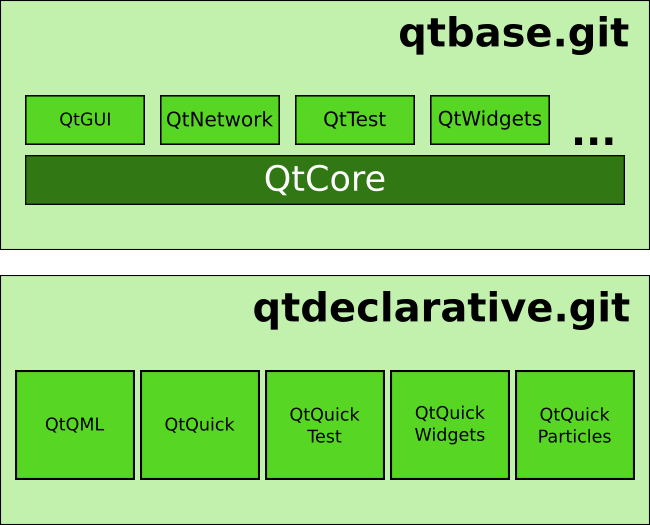
\includegraphics[scale=.66]{qt-repos-and-modules}
    \caption{
        \label{fig:qt-repos-and-modules}
        Qt repository-k és modulok
    }
\end{figure}

Továbbá, Qt 5 óta a modulokat két kategóriába sorolják: \textbf{Qt Essentials} és
\textbf{Qt Add-Ons}. A Qt Essentials-ba tartoznak azok a modulok, amelyek működnek az
összes támogatott platform-on és a legtöbb Qt alkalmazás használja is őket. Ezeknek a
moduloknak az API-ja az 5-ös verzión belül visszafele kompatibilis marad.
A Qt Add-on modulok nem általános célú, "opcionális" modulok. Vannak köztük olyanok,
amelyek nem használhatóak bizonyos Qt által támogatott platformokon vagy olyanok, amelyek
hamarosan eltávolításra kerülnek a Qt keretrendszerből, csak kompatibilitási okokból vannak
még bent (pl. QtScript). A QtWebEngine moduljai is Qt Add-On kategóriába vannak sorolva,
hiszen a legtöbb alkalmazásnak nincs szüksége böngésző funkciókra. API kompatibilitás
szabályait minden Add-On modul saját magának határozza meg.
\cite{bib:qt-doc-qtmodules}

Ha egy Qt-s alkalmazás használ egy Qt modult, akkor azt annak a projekt file-jában
(\texttt{.pro}) meg kell adni:
\begin{verbatim}
    QT += network widgets qml quick
\end{verbatim}
Ez alól kivétel a \texttt{QtCore} és a \texttt{QtGUI} modul. A \texttt{QtCore} modult
minden Qt-s alkalmazás használja, ezért azt a Qt build rendszere implicit linkeli.
Ebben a modulban vannak megvalósítva a Qt típusok és adatszerkezetek, a Qt specifikus nyelvi
elemek és makrók (pl.: \texttt{Q\_OBJECT}, \texttt{signals}, \texttt{slots}),
smart pointerek, stb. A \texttt{QtGUI} modulra a grafikus felhasználói felület
megvalósításához van szükség, de nem kötelező használni (explicit le lehet tiltani).
A \texttt{QtGUI} modulról bővebben a \ref{sec:qt-gui} fejezetben lesz szó.

Ahogy a Qt-s alkalmazások, használnak egy Qt-s modult, úgy a Qt-s modulok is használják
egymást. Az alkalmazáséhoz hasonlóan a modul projekt file-jában is meg kell adni a
függőséget. Továbbá, ha egy komponens modulja használja egy másik komponens modulját, akkor
a komponensek közötti függőséget külön jelezni kell. A függőségek definiálására
``felhasználó'' komponensben van szükség:
\begin{lstlisting}[title=sync.profile]
 %dependencies = (
    "qtbase" => "",
    "qtdeclarative" => "",
    "qtxmlpatterns" => "",
    "qtquickcontrols" => "",
    "qtwebchannel" => "",
 );
\end{lstlisting}

\noindent
Ebben az esetben, a komponensre, mint a modult tároló repository-ra kell
gondolni\footnote{Tovább bonyolítja a helyzetet, hogy sok esetben a komponenseket is
``modul'' elnevezéssel illetjük. Például: ``a QtWebEngine modul függősége a QtBase modul''},
ezért, ha a \texttt{QtCore} modul minden más modul függősége, értelemszerűen az őt tartalmazó
\texttt{QtBase} komponens minden más komponens függősége is lesz, amit ezen a szinten
még explicit meg kell adni.
Az \ref{fig:qtwebengine-dependencies} ábra mutatja, hogy a fenti \texttt{sync.profile} script
alapján a QtWebEngine függőségei hogyan alakulnak.

\begin{figure}[h]
    \centering
    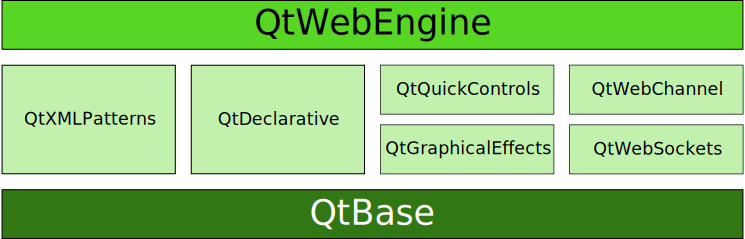
\includegraphics[scale=.66]{qtwebengine-dependencies}
    \caption{
        \label{fig:qtwebengine-dependencies}
        QtWebEngine függőségei
    }
\end{figure}

\subsection{GUI}
\label{sec:qt-gui}
A Qt keretrendszer grafikus felhasználói felületek (GUI) megvalósítására gazdag
eszközkészletet kínál a fejlesztők számára. A QtGUI modul az, amely alacsony szintű API-t
nyújt 2D (rasztergrafika) és 3D (OpenGL API) rajzoláshoz, esemény kezeléshez, képek és
szövegek megjelenítéséhez. A Qt build rendszere automatikusan linkeli ezt a modult az
alkalmazásunkhoz, feltételezvén azt, hogy az úgy is rendelkezik GUI-val. Ha ez nem így
lenne, a QtGUI modul letiltható ha a következő sort adjuk GUI nélküli alkalmazás
projekt file-jához:
\begin{verbatim}
    QT -= gui
\end{verbatim}

Egy grafikus felület megvalósításához nem érdemes csak a QtGUI modult használni. A Qt nyújt
magasabb szintű, QtGUI-ra épülő API-kat is. Jelenleg két egymástól eltérő megközelítés
elérhető: a \textbf{Widget} és a \textbf{Quick}.
\cite{bib:qt-doc-qt-gui, bib:qt-doc-user-interfaces}

\subsubsection{Widget}
A widget API-n keresztül a ``klasszikus'' felhasználói felületeket lehet megvalósítani,
melyeknek megjelenítéséhez a Qt a futtató operációs rendszer stílusát adja\footnote{
\textit{native look'n'feel}}. A widget-ek jellemzően olyan statikus GUI elemek, amelyek
általában desktop-on használt alkalmazások használnak. Megjeleníthetnek vagy tárolhatnak
információt és/vagy felhasználói eseményeket kezelhetnek. Például: gomb (\texttt{QButton}),
címke (\texttt{QLabel}), görgetősáv (\texttt{QScrollBar}), stb. Az a widget, aminek nincs
szülője, az ablak.
\cite{bib:qt-doc-qt-widgets}

A Qt beépített widget-jei a \textbf{QtWidgets} modulból elérhetőek, de saját widget-ek is
készíthetőek. A widget-ek tartalmát a \texttt{QGraphicsView} jeleníti meg. A rajzolás
szoftveresen történik, nincs hardveres gyorsítás.

A QtWidgets modul a widget-eken túl még tartalmaz API-t a widget-ek megjelenítésének
testreszabásához (\texttt{QStyle}) és beépített stílusokat is natív megjelenéshez különböző
platformokon. A widget-ek elrendezésére a beépített \texttt{QLayout} osztályok használhatóak.

A widget alapú GUI-t első sorban \texttt{C++} API-n keresztül lehet felépíteni, de a Qt
keretrendszer tartalmaz egy Qt Designer elnevezésű eszközt is, aminek segítségével,
akár programozási ismeret nélkül össze lehet állítani a GUI-t. A Qt Designer a widget-eket
fába rendezi és XML formátumban tárolja egy \texttt{.ui} kiterjesztésű file-ban. Az XML
file-ból a User Interface Compiler (uic) generál buildelhető \texttt{C++} forrás állományt.

\subsubsection{Quick}
Az új Quick technológia segítségével modern megjelenésű, dinamikus elemekből felépített,
``fluid'' GUI-t lehet összeállítani. Megvalósítás ``deklaratív módszerrel'' történik, ami
magasabb szintű, mint a widget API esetében használatos imperatív paradigma: nem azt kell
leprogramozni, hogyan legyen megjelenítve a GUI, hanem azt, hogy hogyan nézzen ki
(mint például a HTML esetében). A technológia használatához alapvetően 2 modulra van
szükség: \textbf{QtQml}-re és a \textbf{QtQuick}-re.

A Qt egy saját nyelvet nyújt a deklaratív programozáshoz és ez \texttt{QML} (Qt Modeling
Language). Ez a nyelv a \textbf{QtQml} modulon keresztül válik elérhetővé.
A modul rendelkezik \texttt{C++} és \texttt{QML} API-val is, hogy \texttt{QML} nyelv saját
típusokkal és  funkciókkal bővíthető legyen.
A Quick GUI akár ezen a \texttt{C++} API-n keresztül is megvalósítható, de erre a célra
sokkal inkább a \texttt{QML} nyelv használata ajánlott.
A \texttt{QML} nyelv ``JSON-szerű'' szintaxison keresztül írja a UI komponensek
hierarchiáját és kapcsolatait. A \texttt{QML} programot egy külön erre a célra fejlesztett
\texttt{JavaScript} motor dolgozza fel, a \textit{v4}. Ezáltal lehetővé válik, hogy a
UI kódja akár futásidőben is dinamikusan változtatható legyen. \texttt{JavaScript}
kód szabadon hozzáadható a \texttt{QML} forráshoz, így akár logikát is meg lehet valósítani a
\texttt{QML} programon belül. \texttt{JavaScript} használatánál érdemes csak az
eseménykezelésre szorítkozni és a többi vezérlést a QtQml \texttt{C++} API-ján keresztül
\texttt{C++} nyelven megvalósítani.
\cite{bib:qt-doc-qt-qml}

Habár a QtQml modul rendelkezésünkre bocsájtja a \texttt{QML} deklaratív nyelvet, az még
nem rendelkezik olyan elemekkel, amelyekből össze lehetne állítani egy GUI-t. Ezeket a
GUI elemeket \textbf{QtQuick} és a \textbf{QtQuickControls} modulok szolgálgatják.
Majdnem minden elem megtalálható, ami widget API-ban, sőt még több is. További lehetőség
nyílik a felület elemeinek meganimálására QtQuick API-n keresztül.
A QtQuick \texttt{C++} API-ját használva pedig saját \texttt{QQuickItem}-ek hozhatóak létre,
melyek a QtQml API-ján keresztül beregisztrálhatóak a \texttt{QML} nyelvbe.
\cite{bib:qt-doc-qt-quick}

A QtQuick modul felel a Quick GUI elemek megjelenítéséért, kirajzolásáért.
Korábban (QtQuick1) ez ugyanúgy történt, mint a widget esetén, az elemek a \\
\texttt{QGraphicsView}-ra voltak kirajzolva. Ez a megoldás lassú, különösen, ha egy folyton
változó dinamikus felhasználói felületről beszélünk. A jelenleg is használt QtQuick verzióban
(QtQuick2) megjelent a Qt Quick Scene Graph. A Qt Quick Scene Graph a QtQuick modul része,
ezért nem használható önállóan, viszont a modul nyújt hozzá API-t. A scene graph a UI
elemeiből épített fa struktúra, amelyet aztán a modul OpenGL ES 2.0 vagy OpenGL 2.0
API-n keresztül megjelenít. Emiatt a Quick technológia nem használható olyan platformokon,
ahol nem érhető el legalább az OpenGL 2.0 API.
\cite{bib:qt-doc-qt-quick-scene-graph}

\subsection{Web}
A Qt keretrendszerben nem a QtWebEngine az egyetlen komponens/modul ami a
web-hez, web alkalmazásokhoz nyújt API-t.

\subsubsection{QtWebKit}
A QtWebKit a nyílt forrású WebKit böngésző motor portja. Ez a port lecseréli a WebKit-ben
a hálózati kommunikációt és renderelést megvalósító komponenseket a Qt-s megoldásokra és
a WebKit API felé két fajta Qt-s API-t implementál:
\texttt{C++} API-t a Widget alkalmazásokba való beágyazáshoz és \texttt{QML} API-t a Quick
alkalmazásokhoz.
A \texttt{C++} API szinkron, mivel a single-process architektúrájú WebKit API-ra (WebKit1)
épül. Ezzel szemben a Quick integrációt lehetővé tevő \texttt{QML} API aszinkron, mert az már
a multi-process WebKit2-re épül.

A QtWebKit a Qt 4.7-es verziójában jelent meg. A Chromium--WebKit szétválás után a
fejlesztése leállt és csak karbantartási munkákat végeztek rajta. A Qt 5.5-ös release-ben
már elavultnak számít az 5.6-os verzióból már a bináris csomagokat is eltávolították, csak
a QtWebKit forrása elérhető. A QtWebKit leváltására a Chromium-ra épülő QtWebEngine-t
hozták be.

\subsubsection{QtWebView}
A QtWebKit sosem volt támogatott mobil platformokon (Embedded Linuxon igen) és ez jelenleg
hivatalosan igaz a QtWebEngine-re is. Azonban, a mobil platformok (pl. Android, iOS, WinRT)
biztosítanak natív API-t (WebView) a webes tartalmak megjelenítésére, mivel biztonsági
megfontolásból más módon a mobil alkalmazások nem is férhetnének hozzá web tartalomhoz.

A QtWebView modul ezek fölé a natív web API-k felé nyújt wrapper-t és egységes API-t.
Amennyiben nincs elérhető (vagy támogatott) web API a platformon, akkor a QtWebEngine-t
próbálja használni (fallback). A QtWebView-nak csak \texttt{QML} API-ja van.
\cite{bib:qt-doc-qt-webview}

\subsubsection{QtWebSockets}
A WebSocket egy olyan protokoll, amely kétirányú kommunikációt biztosít a web felett.
A kommunikáció kliens és szerver között történik.
A legtöbb modern böngésző integrálja a WebSocket klienst. A QtWebSockets \texttt{C++} és
\texttt{QML} API-t biztosít mind WebSocket kliens és szerver megvalósításához.
\cite{bib:qt-doc-qt-websockets}

\subsubsection{QtWebChannel}
A QtWebChannel modul a Qt 5.4-es verziójában jelent meg. Olyan alkalmazások esetében,
amelyek beépített HTML tartalmat jelenítenek meg szükség lehet olyan megoldásra,
amelynek segítségével a WebView-ban futó web alkalmazás (\texttt{JavaScript}/\texttt{HTML})
és a natív alkalmazás (\texttt{QML}/\texttt{C++}) kommunikálni tud.

A single-process QtWebKit widget API esetén ennek megvalósítása nem jelentett különösebb
problémát, viszont egy multi-process architektúrára épülő motor (WebKit2 vagy Chromium)
a megvalósítás már sokkal bonyolultabb. Erre a problémára nyújt megoldást a QtWebChannel
modul.

A QtWebChannel segítségével Qt MetaObject-et (\texttt{QObject}) lehet ``meghirdetni'' \\
szerver oldalon, a kliens oldal pedig ezt a MetaObject-et tudja használni. \\
A QtWebChannel modul szerver oldalra nyújt \texttt{QML} és \texttt{C++} API-t,
a kliens oldalra pedig \texttt{JavaScript} API-t. A kliens oldalon megjelenő object a
szerver oldali Qt MetaObject másolata, \texttt{JavaScript} API. A két objektum szinkronizálva
van, a property változtatások és a Qt-s szignálok mindkét oldalon megjelennek.

Ez úgy valósul meg, hogy a szerver oldali API szerializálja Qt MetaObject-et majd átküldi
a kliensnek. A kliens oldali API a szerializált Qt MetaObject-ből \texttt{JavaScript}
object-et gyárt, amely képes kommunikálni az eredeti object-el. A kommunikáció történhet
QtWebSockets segítségével, de akár IPC-n keresztül is.
\cite{bib:qt-doc-qt-webchannel, bib:kdab-qt-webchannel}


\subsection{Release}
Egy Qt release verzió száma 3 részből tevődik össze:
\begin{verbatim}
    MAJOR.MINOR.PATCH
\end{verbatim}
A dolgozatomban bemutatott fejlesztések mind az 5-ös főverzióban (\texttt{MAJOR})
jelentek meg. Ahol ez egyértelmű feltüntetem az alverzió számot is (\texttt{MINOR}).
A Qt közösség előre tervezett menetrend szerint fél évente vált alverzió számot (ad ki új
release-t). Dolgozatom készítése idején a Qt 5.6 a legfrissebb stabil kiadás, viszont egyes
bemutatott funkcionalitások, majd csak a Qt 5.7-ben lesznek elérhetőek.

\section{QtWebEngine}
A QtWebEngine váltotta le a QtWebKit-et a Qt keretrendszer 5.4-es verziójában. A célja
megegyezik a QtWebKit-ével: webes tartalom integrálása és manipulálása Qt alkalmazásban.
A QtWebEngine a Chromium-ra épül, pontosabba a Chromium Content Module unstable API-ja
felé implementál egy stable API-t. Az \ref{fig:chromium-architecture} ábra alapján,
a Chrome böngésző alkalmazás helyére a Chromium stack tetején a QtWebEngine kerül és
az lesz a Chromium Content Module-t beágyazó ``alkalmazás''.

A QtWebEngine fejlesztői forkolták a Chromium-ot és ennek a forknak a karbantartása jelentős
nehézséget okoz a QtWebEngine fejlesztőinek. Körülbelül 6 hetente jelenik meg új Chromium
verzió aminek változik az API-ja. Minden új verzió tartalmazhat biztonsági javításokat is,
amelyeket nem backportolnak korábbi verziókba\footnote{A Chromium-nak nincs LTS (Long Term
Support) verziója}, ezért a rendszeres frissítésekre szükség van. Habár amikor csak
lehetséges ezek a javítások cherry-pick-elve vannak a forkba.

A QtWebEngine-nek legnagyobb részét ez a Chromium forknak a kódja teszi ki, habár sok
nem használt Chromium komponens eltávolításra került (pl. Chrome). Viszont egyes
``backend'' komponensek, amelyek lecserélhetőek voltak QtWebKit-ben Qt modulokra, már
nem lecserélhetőek a Chromium-ban. Ilyen például a Chromium network library.

A web elemek kirajzolását viszont a Qt végzi. A mailbox texture azonosítók segítségével a
QtWebEngine hozzáfér a Chrome Compositor által összeállított textúrákhoz, amelyek a
megosztott OpenGL context-en vannak tárolva.
A textúrákból a QtWebEngine épít scene graph fát (\texttt{QSGNode} tree), amit majd a
Qt Quick Scene Graph fog kirajzolni. Emiatt, a Chromium-ban a GPU process ki van kapcsolva,
mert a GPU-t a Qt használja, ami a Browser process-ben fut (\texttt{switches:kInProcessGPU}).

A scene graph függőség miatt a QtWebEngine nem működik olyan környezetben, ahol nincs
OpenGL ES 2.0 vagy OpenGL 2.0. Ez igaz a QtWebEngine Widget API-jára is, mivel a web tartalom
kirajzolásának megvalósítása közös.

A QtWebEngine tartalmazza a QtWebEngine Process-t és 3 modult: a QtWebEngine és a
QtWebEngineWidgets rendre a Quick és Widget API-kat valósítják meg. A QtWebEngineCore
modul tartalmazza a Chromium forkot és QtWebEngine funkcionalitások közös részét, amin a
Quick és a Widget API-k osztoznak. A QtWebEngine felépítését a
\ref{fig:qtwebengine-architecture} ábra mutatja.

\begin{figure}[ht]
    \centering
    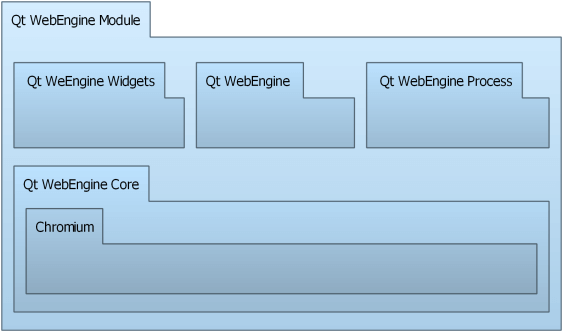
\includegraphics[scale=0.75]{qtwebengine-architecture}
    \caption{
        \label{fig:qtwebengine-architecture}
        QtWebEngine Architecture \cite{bib:qt-doc-webengine-overview}
    }
\end{figure}

\subsection{Process}
A QtWebEngine Process a Chromium Render Process-t fedi el. Különálló program saját belépési
ponttal (\texttt{main()} függvénnyel), amit a Browser Process indít el. Önálló fordítási
egység, de a hozzátartozó kód a QtWebEngine Core modulban van.
Ez processz felel a web tartalom rendereléséért és a \texttt{JavaScript} kódok
végrehajtásáért. A processz OS X-en és Linux-on sandbox-ban fut, Windowson a sandbox
környezet még nem támogatott.

\subsection{Core}
A QtWebEngine Core modul tartalmazza a Chromium fork-ot és implementálja a \\
Chromium Content API interface-eit. Belső (internal) API-ja elfedi a publikus API-k
(Widget, Quick) elől a Chromium Content API-t, így a publikus API-knak nincsenek közvetlen
Chromium függőségeik. A publikus API-k számára közös adapter interface-t \\
(\texttt{WebContentsAdapterClient}) definiál, amit a publikus API-nak kell megvalósítania.

A modul része a Qt Quick Scene Graph integráció is: ő hozza létre a Chromium-ból
kinyert textúrákból a scene graph node-okat (\texttt{QSGNode}) és épít belőle fát a
megjelenítésre (compositing). Továbbá itt található meg a Browser Process és a QtWebEngine
Process inicializációja (\texttt{WebEngineContext}), a QtWebEngine beállításainak továbbítása
a Chromium felé (\texttt{WebEngineSettings}), controller osztályok az API specifikus
dialog ablakok megvalósításához (\texttt{pl.: JavaScriptDialogController}) és még sok minden
más.

Továbbá, QtWebEngine Core modul függősége Qt WebChannel modul, hogy a publikus API-t
használva tetszőlegese saját Qt-s objektum elérhető legyen a weboldal (vagy webalkalmazás)
számára. Ezáltal a fejlesztő hybrid alkalmazást hozhat létre, amelyben a QtWebEngine-el
megjelenített weboldal, kommunikálhat a QtWebEngine-t beágyazó alkalmazással.
A Qt WebChannel Qt WebSockets-ra épülő backend-jét a Qt WebEngine Core cseréli le úgy,
hogy a kommunikáció a Chromium IPC felett történjen, továbbá beregisztrálja a web channel-t
a V8\footnote{a Chromium JavaScript motorja} API-n keresztül az érintett oldal
\texttt{JavaScript} context-jébe.

A Qt 5.6-os verziója óta a Qt WebEngine Core modul rendelkezik publikus API-val is.
Ez az API a Chromium-hoz enged hozzáférést és jellemzően a Widget vagy Quick API-val kell
együtt használni. Ennélfogva a QtWebEngine Core modulját nem szükséges explicit hozzáadni,
a saját Qt-s alkalmazás projektjéhez, mert a Qt WebEngine Widgets és Qt WebEngine (Quick)
modulok automatikusan behúzzák. Ennek az API-nak része a
\texttt{QtWebEngineCore::initialize()} függvény is, amivel a QtWebEngine-t integráló
alkalmazást ``inicializálni'' kell, azért, hogy a megjelenítéshez használt OpenGL context
a processzek között megosztott legyen (\texttt{Qt::AA\_ShareOpenGLContexts}).

\subsection{Widget és Quick API}
A QtWebEngine Widget és Quick API-ját rendre a \\
\textbf{Qt WebEngine Widgets} és \textbf{Qt WebEngine} modulok valósítják meg.
Ezek a modulok nem implementálják vagy hívják közvetlenül a Chromium Content API-t,
hanem azt a Qt WebEngine Core modulon keresztül érik el. A két API között előfordulhatnak
funkcionalitásban előfordulhatnak különbségek, például az egyikben elérhető egy API
függvény a másikban még nem.

A publikus API-k megvalósításánál nagyon fontos szempont a bináris kompatibilitás
biztosítása. Ez nem csak annyit jelent, hogy a meglévő API-k nem változnak, hanem a publikus
(exportált) \texttt{C++} osztályok sem mérete, sem pedig az elrendezése (layout) nem
változhat. Ez a felhasználó számára annyit jelent, hogy saját Qt-s alkalmazása alatt
főverzión belül (esetünkben ez az 5-ös) kicserélheti (frissítheti) a Qt library-t anélkül,
hogy az alkalmazását újra kellene buildelni.

A bináris kompatibilitás megőrzése érdekében a publikus API-k implementálásakor
\textit{d-pointer} (vagy más néven \textit{opaque pointer}) tervezési mintát alkalmazunk.
Ez nem csak a QtWebEngine API-jaira igaz, hanem az összes publikus Qt API-ra is.

A tervezési minta lényege az, hogy az API-ban megvalósított logikát egy rejtett
(\textit{private}) osztály tartalmazza. Az API maga egy másik, publikus (\textit{public})
osztály, ami egy pointer-t tartalmaz rejtett osztályra. Ez a pointer a névadó,
\textit{d-pointer} (private data member). Ezáltal az API implementációja ``rejtve'' marad,
az implementációban módosítások nem változtatják a publikus API-t és publikus API header
file-a átláthatóbb, mert nem tartalmaz olyan metódust vagy adattagot, ami nem a publikus
API része.
\cite{bib:qt-wiki-d-pointer}

\subsubsection{Qt WebEngine Widget}
A Qt WebEngine Widget modul C++ osztályokat nyújt widget GUI létrehozására. Az API
fő komponense a \texttt{QWebEngineView} widget, amely a web tartalom megjelenítésért felel.
Minden \texttt{QWebEngineView} objektumhoz egy \texttt{QWebEnginePage} példány tartozik.
A \texttt{QWebEnginePage} API-n keresztül kérdezhető le és változtatható a web oldal
tartalma.

További API-k: \texttt{QWebEngineHistory} a már látogatott oldalak nyilvántartására és
visszatöltésére, \texttt{QWebEngineProfile} weboldal csoportok kezelésére közös
beállításokkal (pl.: ``inkognitó'' mód: \texttt{QWebEngineProfile::isOffTheRecord()}),
\texttt{QWebEngineSettings} a weboldalak beállításainak kezelésére, \\
\texttt{QWebEngineScript} JavaScript-ek beágyazására.

\subsubsection{Qt WebEngine}
A Qt WebEngine ``fő'' modulja a Quick API. QML típusokat definiál QML/Quick alkalmazások
létrehozására. A nagyjából ugyanazok az API-k állnak rendelkezésre, mint a Widget esetén.
Egy fontos eltérést nem számítva: nincs külön \texttt{WebEnginePage} QML típus az oldal
tartalmának kezelésére, hanem annak API-ja is a \texttt{WebEngineView} QML típusba lett
beépítve.


\chapter{Új funkciók a QtWebEngine-ben}
\label{chap:features}

\todo{Magam csináltam, opensource community -> más is fejlesztett, volt közös munka is
(pl. review)}

\section{Navigation History}

\begin{center}
    \begin{reviewbox}
        \begin{itemize}
            \renewcommand{\labelitemi}{\textcolor{qtgreen}{$\blacktriangleright$}}
            \item \gerrit{81252}
            \item \gerrit{82029}
            \item \gerrit{82380}
            \item \gerrit{81934}
        \end{itemize}
    \end{reviewbox}
\end{center}

\noindent
Az új \textbf{Navigation History} Quick API valósítja meg a böngészési előzmények kezelését,
tárolását. A Widget API már kész volt, ezért az mintaként szolgált, továbbá a Core modulban
a szükséges belső API már meg volt valósítva.

Az alapgondolat az volt, hogy a böngészési előzményeket 2 listában tároljuk az szerint,
hogy az éppen megjelenített oldalnál előbb (\texttt{backItems}) vagy \\
később (\texttt{forwardItems}) lettek betöltve az adott oldalak. Az adatok tárolására
a QML nyelv a \texttt{ListModel} QML típust nyújtja. Az előzmények tárolására specializált \\
\texttt{ListModel}-re van szükség, amit a \texttt{NavigationHistoryListModel} új QML típus
valósít meg. Az új model tárolja az oldalak URL-jét és címét (title), továbbá, lekéri
a látogatott oldalak listáját a Core modul belső API-ján keresztül.

A két \texttt{NavigationHistoryListModel} példány tárolására
egy új Quick Item, a \texttt{NavigationHistory} lett megvalósítva. A Quick Item-eket QML
szinten ugyanúgy ``típusokként'' kezeljük, a különbség mindösszesen annyi, hogy az Item,
a Quick C++ API-jával kerül létrehozásra nem pedig az Qt QML API egy beépített típusának
specializálásával. A \texttt{NavigationHistory} típus (vagy item) tulajdonképpen maga a
böngészési előzményekhez írt API.

%\begin{table}[h!]
\begin{table}[ht!]
    \centering
    \begin{tabular}{ | l | l | p{238pt} | }
        \hline
        \textbf{Property} & \textbf{Típus} & \textbf{Leírás} \\ \hline

        \texttt{backItems} & \texttt{ListModel} &
        Az aktuális oldal előtt látogatott oldalak listája
        \\ \hline

        \texttt{forwardItems} & \texttt{ListModel} &
        Azon oldalak listája, melyek az aktuális oldal után lettek betöltve
        \\ \hline
    \end{tabular}
    \caption{
        \label{tab:navigation-history-history-api}
        Az új \texttt{NavigationHistory} QML típus
    }
\end{table}

Az új QML típusok a Qt QML modul C++ API-jával lettek beregisztrálva a QML nyelvbe, viszont
QML-ből nem példányosíthatóak. Minden \texttt{WebEngineView}-hoz (tab-hoz) tartozik egy
\texttt{NavigationHistory}, ezért azt értelemszerűen a view expliciten példányosítja.
A \texttt{NavigationHistoryListModel} példányok a \\
\texttt{NavigationHistory}-hoz tartoznak, ezért azok azzal együtt jönnek létre.
Ebből kifolyólag, ha hozzáférünk az expliciten példányosított \texttt{NavigationHistory}-hoz,
hozzáférünk a listákhoz is. Az \texttt{NavigationHistory} példányt pedig az azt létrehozó
\texttt{WebEngineView} API-n keresztül érdemes lekérni, de ehhez ezt az API-t is bővíteni
kell.

Ennek a funkcionalitásnak a megvalósításakor, a \texttt{WebEngineView} két API-ra volt
bontva. Volt egy ``mainline'' (maga a \texttt{WebEngineView}) és annak egy ``része'', a \\
\texttt{WebEngineViewExperimental}. A \texttt{WebEngineViewExperimental} egy ``kísérleti''
API, ami olyan funkcionalitásokat nyújtott, amelyek újak és még véglegesítésre várnak
(ezért unstable API), vagy pedig csak a teszteléshez szükségesek (nem javasolt a használata).
Ez a módszer Qt WebKit-ből került át, viszont a legújabb Qt WebEngine verziókban
próbálunk a \texttt{WebEngineViewExperimental} API-tól megszabadulni, ezért abba már nem
kerülnek új funkcionalitások, továbbá dokumentálva sincsen.

Mivel a \texttt{NavigationHistory} még a Qt WebKit-ben is kísérleti API volt, ezért az a
Qt WebEngine-ben is csak a \texttt{WebEngineViewExperimental} API-n keresztül vált
elérhetővé. Mivel önmagában az előzmények kilistázásának nem sok haszna van, ezért a view
API-hoz további funkcionalitások lettek hozzáadva, amelyek a már látogatott oldalak
újratöltését tették könnyebbé. Ezek listája a \ref{tab:navigation-history-experimental-api}
táblázatban látható.

\begin{table}[h!]
    \centering
    \begin{tabular}{ | l | l | p{194pt} | }
        \hline
        \textbf{Property} & \textbf{Típus} & \textbf{Leírás} \\ \hline

        \texttt{navigationHistory} & \makecell[l]{\texttt{Navigation} \\ \texttt{History}} &
        \makecell[l]{Az aktuális view-hoz tartozó \\ \texttt{NavigationHistory} példány}
        \\ \hline

        \makecell[l]{\texttt{currentNavigation} \\ \texttt{EntryIndex}} & \texttt{int} &
        Az aktuális oldal indexe a history-ban
        \\ \hline

        \texttt{goBackTo(int)} & \texttt{slot} &
        \makecell[l]{A paraméterben átadott index-el lép \\
                     vissza a \texttt{backItems} listában és \\
                     tölti be az oldalt}
        \\ \hline

        \texttt{goForwardTo(int)} & \texttt{slot} &
        \makecell[l]{A paraméterben átadott index-el lép \\
                     előre a \texttt{forwardItems} listában és \\
                     tölti be az oldalt}
        \\ \hline
    \end{tabular}
    \caption{
        \label{tab:navigation-history-experimental-api}
        Új funkciók a \texttt{WebEngineViewExperimental} QML típusban
    }
\end{table}

Az új funkciók tesztelésére a Qt WebKit-ben is használt teszt lett portolva a \\
Qt WebEngine-be és további teszt esetekkel lett kibővítve a lefedettség javítására.
A tesztelés módszere, hogy a \texttt{WebEngineView} API segítségével navigálunk oldalak
között és minden (sikeres) oldal betöltés után ellenőrizzük a \texttt{NavigationHistory}-ben
tárolt listák méretét.

A fent bemutatott funkció a Qt 5.4-es verziójában jelent meg a Qt WebEngine bekerülésével
együtt a kísérleti API részeként. A cél az volt, hogy a Qt WebKit \\
\texttt{NavigationHistory} megvalósítása legyen átültetve a Qt WebEngine-be a lehető
legkevesebb API módosítással.
A Qt 5.5-ös verzióban ez az API már a ``mainline'' API-ba került át, jelentős
változtatásokkal az API-n. A legnagyobb eltérés, hogy a QML típusok esetén a
\texttt{NavigationHistory} elnevezést/prefixet \texttt{WebEngineHistory}-ra cseréltük,
viszont a \texttt{WebEngineView.navigationHistory} property elnevezés megmaradt, visszafele
kompatibilitási okokból.


\section{Find Text}

\begin{center}
    \begin{reviewbox}
        \begin{itemize}
            \renewcommand{\labelitemi}{\textcolor{qtgreen}{$\blacktriangleright$}}
            \item \gerrit{91117}
        \end{itemize}
    \end{reviewbox}
\end{center}

\noindent
A Navigation History-hoz hasonlóan a \textbf{Find Text} is már meg volt valósítva a Widget
API-ban ezért csak a Quick API-t kellett megvalósítani a Qt WebKit implementációja alapján.
A funkció lényege, hogy adott szöveget keressen meg az oldalon, a legközelebbi előfordulást
emelje ki a view-ban, és legyen lehetőség találat esetén az esemény kezelésre.

Ehhez a funkcióhoz elegendő egyetlen függvényt hozzáadni az API-hoz és ez a \\
\texttt{findText}. Mivel a keresést a view-ban kirenderelt szövegen kell végrehajtani,
ezért értelemszerűen \texttt{WebEngineView} API része kell, hogy legyen. Mivel, a
\texttt{findText} is kísérleti funkcióként kezdte, ezért először a
\texttt{WebEngineViewExperimental} API-hoz lett hozzáadva a \ref{tab:find-text-api}
táblázatban látható módon.

\begin{table}[h!]
    \centering
    \begin{tabular}[t]{ | l | l | p{188pt} | }
        \hline
        \textbf{Property} & \textbf{Típus} & \textbf{Leírás} \\ \hline

        \makecell[l]{\texttt{findText(substring,} \\
                     \texttt{~~~~~~~~~options,} \\
                     \texttt{~~~~~~~~~callback)}} & \texttt{slot} &
        \makecell[l]{Megkeresi \texttt{substring}-et az oldalon, \\
                     az \texttt{options} beállítások szerint. \\
                     Találat esetén meghívódik a \\
                     \texttt{callback} függvény (JavaScript)}
        \\ \hline

        \texttt{FindBackward} & \makecell[l]{\texttt{FindFlags} \\ \texttt{(enum)}} &
        \makecell[l]{\texttt{findText} beállítás: az oldalon \\
                     visszafele keres}
        \\ \hline

        \texttt{FindCaseSensitively} & \makecell[l]{\texttt{FindFlags} \\ \texttt{(enum)}} &
        \makecell[l]{\texttt{findText} beállítás: a keresésben \\
                     kis és nagy betűket megkülönbözteti}
        \\ \hline
    \end{tabular}
    \caption{
        \label{tab:find-text-api}
        Új funkciók a \texttt{WebEngineViewExperimental} QML típusban
    }
\end{table}

A megvalósításhoz ismét a már meglévő belső Core API-t kellett használni a következő módon:
a \texttt{WebEngineViewExperimental::findText} függvény meghívja
a \texttt{WebContentsAdapater::findText} függvényt a Core-ban,
annak átadja a keresett stringet és megfelelő formában a keresés ``konfigurációját'',
ha a keresett string nem üres.
Ha üres, akkor megállítja az éppen futó kereséseket és meghívja a paraméterben
megadott callback függvényt (ha van), azzal az eredménnyel, hogy 0 egyezést talált.

Ha a \texttt{WebContentsAdapater::findText} függvényt hívta, akkor az egy azonosítóval
tér vissza (\texttt{requestId}), amire a callback függvény beregisztrálásához van szükség.
A callback függvény használata opcionális, amennyiben nincs megadva az azonosító nem lesz
beregisztrálva. A \texttt{WebEngineView} API közös\footnote{más API függvényeknek is lehet
callback-je, pl.: \texttt{runJavaScript}} tárolót (map-et) definiál a callback függvények
tárolására, ahol a kulcs az azonosító, az érték a JavaScript callback függvény:
\begin{verbatim}
    QMap<quint64, QJSValue> m_callbacks;
\end{verbatim}
A keresés aszinkron történik (párhuzamosan a render processzben), ezért a \\
\texttt{didFindText} függvény itt véget ér és nem ad vissza semmilyen eredményt. Ha volt
beállítva callback függvény akkor a fejlesztő azon keresztül értesül a találatról, különben
a megtalált szöveg a view-ban lesz kiemelve. Amint a Chromium befejezte a keresést a
Content API-n keresztül értesíti a WebEngine Core-t, ami pedig az API-ban meghívja a
\texttt{WebEngineViewExperimental::didFindText} függvényt. Ez a függvény kikeresi a
paraméterében kapott azonosító a alapján a beregisztrált callback függvényt és meghívja azt.

A JavaScript callback függvénynek egy paramétere van, ami a találatok \\
száma (\texttt{matchCount}). Ha ez a paraméter 0, akkor a keresés sikertelen volt.
Tervben van a callback függvény kiegészítése egy második, az úgy nevezett \\
\texttt{activeMatchOrdinal} paraméterrel is, ami azt mondja meg, hogy az összes találat
közül melyik van éppen kiemelve. Minden újabb \texttt{findText} hívással, amelyben nem
változik a keresett string , a következő találat lesz kiemelve és az \\
\texttt{activeMatchOrdinal} értéke nő eggyel, amíg a keresés körbe nem ér.
Ez a funkció, azért nem lett megvalósítva a Qt WebEngine-ben, mert mikor
ez az implementáció készült, a Chromium \texttt{activeMatchOrdinal} funkciója hibás volt.

Az új funkcióhoz a tesztek a QtWebKit-ből lettek áthozva és átalakítva úgy, hogy
támogassák az új callback alapú API-t (a QtWebKit API-ja signal-okkal jelezte, ha van
találat). A tesztelés során azt ellenőrízük, hogy különböző oldalakon a \texttt{findText}
megfelelő darabszámú egyezést talált-e. Továbbá, az új API függvény be lett építve a
Qt WebEngine teszt böngészőjébe (quicktestbrowser), ahol \texttt{Ctrl+f} billentyű kombináció
hatására felugrik egy felület a kereséshez, ahol keresést lehet indítani, megszakítani és
oda-vissza navigálni a találatok között.

Ez a kísérleti funkció a Qt WebEngine-el együtt jelent meg a Qt 5.4-ben, majd a Qt 5.5-ben
került át a mainline API-ba minimális változtatással és dokumentációval.


\section{Log Level}

\begin{center}
    \begin{reviewbox}
        \begin{itemize}
            \renewcommand{\labelitemi}{\textcolor{qtgreen}{$\blacktriangleright$}}
            \item \gerrit{94266}
        \end{itemize}
    \end{reviewbox}
\end{center}

\noindent
A \textbf{Log Level} funkció esetében nem egy új API-ról vagy egy meglévő bővítéséről van
szó, hanem egy új kapcsoló a \texttt{-{}-log-level=[0123]} hozzáadásáról a Qt WebEngine-hez.
Az új funkció természetéből adódóan nincs szükség/lehetőség tesztelésre sem.

Az új kapcsolóra azért volt szükség, mert a Qt WebEngine-t beépítő alkalmazások rengeteg
üzenetet írtak ki a konzolra, ami a Chromium-tól jött. Ezeknek túlnyomó része lényegtelen
információ a QtWebEngine-t használó fejlesztő számára, ezért az elsődleges cél ezek
letiltása volt. Viszont hibakeresés szempontjából fontosak lehetnek a hibaüzenetek a
fejlesztés során, ezért egy kapcsolóra volt szükség, ami ezt szabályozza.

Az üzenetek szűrésére a Chromium naplózási szinteket definiál:
\begin{description}[
            labelsep=-0.5cm,
            itemsep=0cm,
            before={\renewcommand\makelabel[1]{\bfseries ##1}}]
    \item[0] \texttt{LOG\_INFO}
    \item[1] \texttt{LOG\_WARNING}
    \item[2] \texttt{LOG\_ERROR}
    \item[3] \texttt{LOG\_FATAL}
\end{description}
Ezek közül a Qt WebEngine szempontjából csak a \texttt{LOG\_FATAL} szintű üzenetek
relevánsak, tehát minimum log szintnek ezt kell beállítani. \\
Erre szolgál a Chromium \texttt{logging::SetMinLogLevel} függvénye:
\begin{verbatim}
    int logLevel = logging::LOG_FATAL;
    logging::SetMinLogLevel(logLevel);
\end{verbatim}
A \texttt{logging::SetMinLogLevel} függvény, nem a Content API része, hanem a \\
Chromium base modulé, továbbá a Qt-s üzenetekre semmilyen hatással nincsen. \\
A \texttt{-{}-log-level} kapcsoló segítségével, ezt a minimum szintet lehet
parancssorból felüldefiniálni. A kapcsoló is a Chromium része, a
\texttt{switches::kLoggingLevel} azonosítóval lehet rá hivatkozni:
\begin{verbatim}
    std::string logLevelValue = parsedCommandLine->
    GetSwitchValueASCII(switches::kLoggingLevel);
\end{verbatim}

A megvalósítás során a legnagyobb kihívást a függvény megtalálása jelentette, ahol a minimum
log szintet mind a browser, mind a render processzekre be lehet állítani.
A választás a \texttt{ContentMainDelegate::PreSandboxStartup} függvényre esett, mivel
meghívódik a browser processzben és a render processzben is a sandbox inicializáció előtt,
továbbá a Chromium Content API-n keresztül felüldefiniálható.

A \texttt{-{}-log-level} kapcsoló a Qt WebEngine-el együtt jelent meg a Qt 5.4-es
verziójában.


\section{Test Support API}

\begin{center}
    \begin{reviewbox}
        \begin{itemize}
            \renewcommand{\labelitemi}{\textcolor{qtgreen}{$\blacktriangleright$}}
            \item \gerrit{107089}
        \end{itemize}
    \end{reviewbox}
\end{center}

\noindent
A \textbf{Test Support API} kimondottan csak tesztelésre lett létrehozva: olyan funkciók
érhetőek el innen, amit szándékozunk a publikus API részévé tenni, mert a fejlesztőknek
nincs rá szüksége, viszont bizonyos publikus API funkciók teszteléséhez elengedhetetlenek.
Ebből kifolyólag dokumentálva sincsen.
Ez az API csak QML tesztekhez lett megvalósítva, mivel a Qt WebEngine az elsődleges API
és Widget oldalon könnyebb a tesztelés. \\
Másodlagos cél a \texttt{WebEngineViewExperimental} API fokozatos kiváltása volt.

A teszt, ami behozta ezt az új API-t az \textit{Error Page}-ket tesztelte.
Ez a funkció sikertelen oldal betöltés esetén egy beépített oldalt jelenít meg a
hibaüzenettel, ami maga az \textit{Error Page}. A tesztelés azon alapul, hogy a sikeres és
sikertelen oldal betöltések befejezése után a WebEngineView signal-t küld:
\texttt{loadingChanged}. A \textit{Error Page} esetén arra számítunk, hogy ennek a signal-nak
a paramétere hibás oldal betöltésének adatait tárolja. A gond az, hogy a \textit{Error Page}
is oldal, tehát küld signal-t, ha sikeresen betöltődött.

Kézenfekvőnek tűnik a megoldás, hogy ne küldjük az \textit{Error Page} töltését jelző
signal-okat, és akkor csak a hibás oldal betöltésének signal-jait kapjuk meg. Ezzel a gond
az, hogy a tesztbe új oldalt betöltést csak úgy kezdhetünk, ha az \textit{Error Page}
betöltése már befejeződött, amit signal-ok nélkül nem tudunk ellenőrizni.

Másik lehetőségként merült fel, hogy a hibás oldal, hibát jelző \texttt{loadingChanged}
signal-ját csak akkor küldjük el, miután az \texttt{Error Page} is betöltődött. Ez további
problémákat vet fel: nem tudjuk tesztelni, hogy az \texttt{Error Page} betöltése sikeres
volt e (szélsőséges esetben az \texttt{Error Page} betöltése is meghiúsulhat),
illetve, ha a felhasználó megszakítja az \texttt{Error Page} betöltését, az API nem értesít
arról, hogy történt egy hibás oldal betöltés. Továbbá, oldal betöltés során érkeznek más
signal-ok is (pl.: hány százalékon áll az oldal töltése), aminek lekezelés ebben az esetben
túl sok hiba lehetőséget hordozna magában.

Végül az első változat lett megvalósítva: a hibás oldal signal-jai változtatás nélkül
elérhetőek a publikus API-n keresztül, de az \textit{Error Page} signal-jai nem, azt csak
egy belső, tesztelésre szánt API-n keresztül lehet elérni. Ez lett a
\textbf{Test Support API}. Az új API-val megoldható lett az, hogy tesztelés során, minden
\texttt{loadingChanged} signal-t elkapjunk, a hozzátartozó \texttt{LoadRequest}-et egy
listában tároljuk és a lista elemeit bejárva ellenőrizzük, hogy megfelelő oldal betöltések
történtek e, a megfelelő sorrendben.

\begin{table}[h!]
    \centering
    \begin{tabular}{ | l | l | p{185pt} | }
        \hline
        \textbf{Property} & \textbf{Típus} & \textbf{Leírás} \\ \hline

        \makecell[l]{\texttt{loadingChanged} \\ \texttt{(WebEngineLoadRequest)}} &
        \texttt{signal} &
        \makecell[l]{
        Ez a signal lesz kiküldve amikor az \\
        oldal betöltése megkezdődik, befeje-\\
        ződik vagy hiba miatt megszakad}
        \\ \hline
    \end{tabular}
    \caption{
        \label{tab:test-support-webengine-errorpage}
        Az új \texttt{WebEngineErrorPage} QML típus
    }
\end{table}

\begin{table}[h!]
    \centering
    \begin{tabular}{ | l | l | p{195pt} | }
        \hline
        \textbf{Property} & \textbf{Típus} & \textbf{Leírás} \\ \hline

        \texttt{errorPage} & \texttt{WebEngineErrorPage} &
        \makecell[l]{
            \texttt{WebEngineErrorPage} példány, \\
            a \texttt{WebEngineView}-ba betöltött \\
            \textit{Error Page} \texttt{loadingChanged} \\
            signal-jának elkapására}
        \\ \hline
    \end{tabular}
    \caption{
        \label{tab:test-support-webengine-testsupport}
        Az új \texttt{WebEngineTestSupport} QML típus
    }
\end{table}

Az API megtervezése után a következő kihívást annak kitalálása jelentette, hogy
hogyan tegyük elérhetővé, a Test Support API-t. Nyilvánvaló, hogy valamilyen módon,
a \texttt{WebEngineView}-hoz kell kötni. A legkézenfekvőbb megoldásnak a \\
\texttt{WebEngineView} QML típus kiterjesztése tűnt. Erre a \\
\texttt{qmlRegisterExtendedType()} függvény nyújt lehetőséget, ami a Qt QML C++ API része.
A \texttt{WebEngineView} ugyanezzel a megoldással van kiterjesztve az Experimental
API-val. Ez viszont nem működött, mivel egy ismert, de még nem javított hiba miatt,
egy QML típust, csak egy másik típussal lehet kiterjeszteni, mert a rákövetkező típus mindig
felülírja az előzőt. Ez azt jelenti, hogy az ha az Experimental és a Test Support API is
kiterjesztésként van beregisztrálva, egy QML programban egyszerre csak az egyik
használható.

Így Test Support API (az Experimental API-val való ütközést elkerülendő), önálló,
példányosítható QML típusként lett megvalósítva. Az összeköttetést a \\
\texttt{WebEngineView}-al a \texttt{WebEngineView} API kibővítésével lett megoldva: \\
a \texttt{testSupport} property-n keresztül beregisztrálható az explicit létrehozott \\
\texttt{WebEngineTestSupport} példány, a \texttt{WebEngineView} pedig, ha rendelkezik
ilyen példánnyal, akkor a megfelelő eseményeket át fogja irányítani neki.

\begin{table}[h!]
    \centering
    \begin{tabular}{ | l | l | p{216pt} | }
        \hline
        \textbf{Property} & \textbf{Típus} & \textbf{Leírás} \\ \hline

        \texttt{testSupport} & \texttt{WebEngineView} &
        \makecell[l]{
            Ezen a property-n keresztül regisztrálható \\
            be az explicit példányosított \\
            \texttt{WebEngineTestSupport} példány}
        \\ \hline
    \end{tabular}
    \caption{
        \label{tab:test-support-webengine-view}
        Az új \texttt{WebEngineTestSupport} QML típus
    }
\end{table}

Az ellenőrzés, hogy van e beregisztrált Test Support API többlet költséggel jár, ráadásul
egy átlag fejlesztőnek nincs is rá szüksége. Ezért a Test Support-hoz tartozó kódok az
\texttt{ENABLE\_QML\_TESTSUPPORT\_API} makróval lettek guard-olva. Ha Qt úgy lett
konfigurálva, hogy ne buildeljen teszteket (ahogy release esetén is), akkor a Test Support
API le lesz tiltva és nem lesz lebuildelve. Ha a fejlesztő később mégis lebuildelné a
QML teszteket, akkor a build rendszer figyelmeztet, hogy a Test Support API le van tiltva
és segítséget nyújt, hogyan lehet engedélyezni és lebuildelni.

A \textbf{Test Support API} Qt 5.5-ös verziójában jelent meg.


\section{Form Validation}

\begin{center}
    \begin{reviewbox}
        \begin{itemize}
            \renewcommand{\labelitemi}{\textcolor{qtgreen}{$\blacktriangleright$}}
            \item \gerrit{107066}
            \item \gerrit{122727}
        \end{itemize}
    \end{reviewbox}
\end{center}

\noindent
A \textbf{Form Validation} egy HTML5 funkció, amely HTML-ben írt ``űrlapok'' beviteli
mezőit ellenőrzi scriptek nélkül: ki lett e töltve a beviteli mező, e-mail vagy URL
formátumú-e a bevitt adat, stb. A feltételeket az input tag-en belül kell megadni és
egyéni minták is definiálhatóak. Ha az input mezőbe bevitt adat nem felel meg a
kívánalmaknak, az űrlap elküldése (\textit{submit}) helyett a böngésző felugró buborékban
(\textit{Message Bubble}) jelzi a hiba okát.

Ez a funkció meg van valósítva a Chromium-ban, viszont a hibaüzenet megjelenítését, már
a beágyazó alkalmazásra bízza. A Qt WebEngine nem támogatta sem a hibaüzenet továbbítását
API-n keresztül, sem pedig az üzenet megjelenítését egyik modulban sem. A funkció új API
helyett \texttt{UI Delegate}-el lett megvalósítva Qt WebEngine és Qt WebEngine Widgets
modulokban. \texttt{UI Delegate} esetén nem a fejlesztőnek kell lekezelni az eseményt és
megjelenítenie egy UI elemet, hanem annak megvalósítása már a Qt WebEngine része.

A Chromium Content API 3 callback függvénnyel jelzi, hogy ha a megjelenítendő üzenet állapota
változik:
\begin{description}
    \item[\texttt{ShowValidationMessage}] Az üzenetet meg kell jeleníteni
    \item[\texttt{HideValidationMessage}] Az üzenetet el kell rejteni
    \item[\texttt{MoveValidationMessage}] Az üzenet pozíciója megváltozott a képernyőn
\end{description}
Ezek a függvények a Core modulban meg lettek valósítva úgy, hogy a \\
\texttt{WebContentsAdapterClient} megfelelő függvényeit hívják meg, paraméterben
a megjelenítéshez szükséges adatokat Qt-s típusokra konvertálva. Mindkét modul
szövegbuborékot rajzol, benne a hibaüzenettel a hibás input mező alá.

\begin{figure}[h]
    \centering
    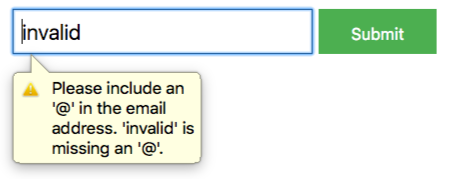
\includegraphics[scale=0.75]{bubi-widget-screenshot}
    \caption{
        \label{fig:bubi-widget-screenshot}
        \texttt{QtWebEngineWidgetUI::MessageBubbleWidget}
    }
\end{figure}

A Qt WebEngine Widgets modulban új widget lett megvalósítva a szövegbuborék számára:
\texttt{MessageBubbleWidget}. Az új widget a \texttt{QtWebEngineWidgetUI} névtérből
elérhető és csak a Qt WebEngine számára. Az új névtér a \texttt{UI Delegate}-ként szolgál
a Qt WebEngine Widgets modulban. Qt WebEngine-hez tartozó \texttt{UI Delegate}-nek fordítási
időben letilthatónak kell lennie, ezért az itt implementált funkciók nem lesznek részei
a Qt WebEngine-nek, ha a projekt a \texttt{WEBENGINE\_CONFIG=no\_ui\_delegates} beállítással
van konfigurálva.

A \texttt{MessageBubbleWidget} singleton-ként van tárolva \texttt{UI Delegate}-en belül,
így nem kell mind üzenethez újra felépíteni a widget-et, csak újra rajzolni. Hozzáférést
az alábbi belső API szolgáltat:
\begin{itemize}
    \item \texttt{QtWebEngineWidgetUI::MessageBubbleWidget::showBubble(} \\
                    \texttt{view, anchor, mainText, subText)}
    \item \texttt{QtWebEngineWidgetUI::MessageBubbleWidget::hideBubble()}
    \item \texttt{QtWebEngineWidgetUI::MessageBubbleWidget::moveBubble(} \\
                    \texttt{view, anchor)}
\end{itemize}
A \texttt{view} (\texttt{QWebEngineView}) paraméterre azért van szükség, hogy a buborék
pozíciója meghatározható legyen az ablakon belül. Az \texttt{anchor} (\texttt{QRect}) annak
a HTML elemnek (beviteli mezőnek) ``körvonala'', amelynek a tartalma a hibát kiváltotta.
Ez arra van használva, hogy a buborék méretét kiszámítsuk. A \texttt{mainText}
(\texttt{QString}) maga a hibaüzenet, míg a \texttt{subText} (\texttt{QString)} HTML mező
azonosítója ha az meg van adva. Maga buborék \texttt{QPainter}-el lett megrajzolva, a bal
felső sarokban található ikon pedig a Qt standard, üzenet mezőhöz tartozó ikonja.

\begin{figure}[ht]
    \centering
    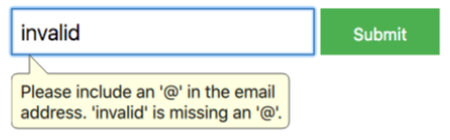
\includegraphics[scale=0.75]{bubi-quick-screenshot}
    \caption{
        \label{fig:bubi-quick-screenshot}
        \texttt{MessageBubble} QML típus
    }
\end{figure}

A Qt WebEngine modul szövegbuborékja mind megvalósítása, mind megjelenítése némileg eltér
a widget-es szövegbuboréktól. A szövegbuborék tárolásáról és annak eléréséről
\texttt{UIDelegatesManager} osztály gondoskodik:
\begin{itemize}
    \item \texttt{UIDelegatesManager:showMessageBubble(} \\
                    \texttt{anchor, mainText, subText}
    \item \texttt{UIDelegatesManager::hideMessageBubble()}
    \item \texttt{UIDelegatesManager::moveMessageBubble(anchor)}
\end{itemize}
A két API többé kevésbé megegyezik. A legfontosabb különbség, hogy itt nem kell átadni a
\texttt{view}-t paraméterül, mert az a \texttt{UIDelegatesManager} adattagja. A szövegbuborék
QML típus QML nyelven lett megvalósítva: \texttt{MessageBubble.qml}. A buborék
megrajzolás a \texttt{Canvas} QML típus segítségével történik. A \texttt{Canvas} típus
ugyanolyan JavaScript API-t nyújt a rajzoláshoz, mint a HTML5 \texttt{Canvas} elem.
Sajnos ikon használatára nem volt lehetőség, mivel a Qt a QML nyelvben nem nyújt beépített
ikonokat sem pedig ikon támogatást. A widget-es ikonok használatát kerülni kellett, mert
a Qt WebEngine modul-nak nem lehet Qt Widgets függősége.

Az Form Validation funkció tesztelésére a Test Support API lett felhasználva. Mivel a
Qt WebEngine-ben a Form Validation-nek nincs publikus API-ja a hiba üzeneteket a
Test Support API teszi elérhetővé a tesztek számára a \\
\texttt{QQuickWebEngineTestSupport::ValidationMessageShown}
signal-on keresztül. A hibásan kitöltött űrlapok ellenőrzéséhez az elküldés (submit) gomb
megnyomására is szükség van a tesztekben. A teszt a gomb megnyomására felhasználói interakció
híján a Qt Test modul \texttt{keyPress()} függvényét használja. A megfelelő gomb
kiválasztását (``fókuszálását'') JavaScript kód végzi, ahol a megfelelő gomb azonosítóját
az URL fragment tartalmazza.

A Form Validation HTML5 funkció támogatása és a hozzátartozó szöveg buborékok a Qt 5.5-ös
verzióban jelentek meg. A funkció tesztelése már csak az 5.6-os verzióba került be.

\pagebreak
\section{Localization}

\begin{center}
    \begin{reviewbox}
        \begin{itemize}
            \renewcommand{\labelitemi}{\textcolor{qtgreen}{$\blacktriangleright$}}
            \item \gerrit{110958}
            \item \gerrit{111004}
        \end{itemize}
    \end{reviewbox}
\end{center}

\noindent
A \textbf{Localization} funkció felel a Chromium üzeneteinek (legyen az hiba üzenet vagy
a Form Validation funkció üzenete) lefordításáért. Alapértelmezetten az üzenetek a
rendszer szinten beállított nyelven fognak megjelenni. Ez a nyelv felüldefiniálható
a render processzben a Chromium \texttt{-{}-lang} kapcsolóval. A browser processzben
ugyanerre a célra a Content API \texttt{ContentBrowserClient::GetApplicationLocale()}
függvényén keresztül van lehetőség.

Tesztelésnél kulcsfontosságú, hogy az üzenetek angol nyelven jelenjenek meg, mivel a
tesztelés során angol nyelvű hiba üzeneteket használjuk referenciaként. A Chromium
alapértelmezett nyelvét a Qt által használt nyelvi beállításokkal definiáltuk felül:
\begin{verbatim}
std::string ContentBrowserClientQt::GetApplicationLocale()
{
    return QLocale().bcp47Name().toStdString();
}
\end{verbatim}
Ez alapján, ahhoz, hogy a tesztekben angol nyelvű hibaüzenetek kapjunk elég a Qt API-n
keresztül beállítani a nyelvet, a tesztelés inicializálásakor:
\begin{verbatim}
QLocale::setDefault(QLocale("en"));
\end{verbatim}
Ez a megoldás azonban nem működött és erről hiba jelentés (bug report) is készült:
\begin{center}
    \begin{issuebox}
        \begin{itemize}
            \renewcommand{\labelitemi}{\textcolor{qtred}{$\blacktriangleright$}}
            \item \qtbug{45715}
        \end{itemize}
    \end{issuebox}
\end{center}

A hiba oka a Chromium-ban volt, ezért a javítást a \textit{qtwebengine-chromium} Chromium
forkhoz kellett hozzáadni. A probléma az volt, hogy amelyik rendszeren volt elérhető
GLib ott arra volt bízva a megfelelő lokalizáció kiválasztása. Qt esetében ezt a kód részt
(``code path''-t) ki kellett kapcsolni, hogy ne írja felül a Qt beállításait.

Egyes üzenetek a render processztől jönnek, amelyekre nem érvényes a \\
\texttt{ContentBrowserClient::GetApplicationLocale} beállítása. A render processznek
és más nem browser processzeknek van egy \texttt{-{}-lang} parancssori kapcsolója, amivel
megadható a kiválasztott locale. A Content API \\
\texttt{ContentBrowserClientQt::AppendExtraCommandLineSwitches()} \\
függvényének implementálásával megadható, hogy amikor a browser processz új processzt indít,
annak milyen kapcsolót adjon át. Így ezzel a megoldással minden újonnan induló processznek
átadjuk a \\
\texttt{ContentBrowserClient::GetApplicationLocale()} függvény által visszaadott
locale-t a processz \texttt{-{}-lang} kapcsolóján keresztül:
\begin{verbatim}
AppendSwitchASCII(switches::kLang, GetApplicationLocale());
\end{verbatim}

Ezzel a megoldással a tesztekben kapott Chromium üzenetek minden esetben angolul jelenik meg,
viszont előfordulhat, hogy a felhasználó is szeretné felül definiálni parancssorból a
böngésző alkalmazás nyelvét, ezért a Qt WebEngine-ben a browser processzben is meg lett
valósítva, hogy \texttt{-{}-lang} kapcsolóval átadott érték felülírja a Qt alapértelmezett
nyelvi beállítását. \\
Ez a \texttt{WebEngineLibraryInfo::getApplicationLocale()} függvényben
lett megvalósítva, hogy ha a browser processz \texttt{-{}-lang} kapcsolóval lett indítva,
akkor annak az értékével térjen vissza és ne kérje le a Qt-tól a locale értékét.

Az új \texttt{-{}-lang} parancssori kapcsoló támogatása és a tesztelés javítása a Qt 5.5-ös
verziójában jelent meg.


\section{Authentication Dialog}

\begin{center}
    \begin{reviewbox}
        \begin{itemize}
            \renewcommand{\labelitemi}{\textcolor{qtgreen}{$\blacktriangleright$}}
            \item \gerrit{124330}
            \item \gerrit{124331}
            \item \gerrit{124332}
            \item \gerrit{124333}
        \end{itemize}
    \end{reviewbox}
\end{center}

\noindent
Az legtöbb böngésző támogatja a HTTP protokoll által nyújtott bejelentkezés funkciót
(Basic Access Authentication - RFC 2617), amely a legegyszerűbb módja a web lapok jelszóval
való védésének. Nincs szükség bejelentkező oldalra, cookie-kra, hanem a HTTP header
megfelelő mezőit használja az azonosításhoz. Továbbá HTTP protokoll támogatja a HTTP proxy
szerverre történő bejelentkezést is.

A HTTP protokollon keresztül történő bejelentkezéshez szükséges form (űrlap) nem a web
oldalon jelenik meg, ezért azt jellemzően a böngészők egy felugró ablakon teszik láthatóvá
a felhasználó számára. A Chromium megvalósítja a HTTP protokollon keresztül történő
bejelentkeztetést, viszont a felugró ablakot a beágyazó alkalmazásnak kell megvalósítania
a Content API-n keresztül. A Qt WebEngine ezt megvalósító funkciója az
\textbf{Authentication Dialog}.

Az Authentication Dialog már meg volt valósítva a Qt WebEngine Widgets modulban, azonban
ez a megvalósítás hibás volt, illetve az ehhez tartozó implementáció a Core modulban nem
volt felhasználható egy Quick UI Delegate megvalósításához. A Quick funkció megvalósítását
ezért a Widget API javításával és újraírásával kezdtem.

Az első kijavítandó hiba az volt, hogy a Widget megvalósítás nem támogatta az üres
felhasználónév és jelszó párral történő bejelentkezést, mivel ezt az esetet úgy kezelte,
hogy a felhasználó megszakítja a bejelentkezést (Mégse/Cancel gomb). A felhasználó név
és jelszó (credentials) tárolására a Qt Network module saját osztályt definiál:
\texttt{QAuthenticator}. A hiba javításához megszakítás esetén a \texttt{QAuthenticator}
példány \texttt{user} és \texttt{password} mezőjébe nem üres string-et tárolunk, hanem
nem állítunk be semmit és a példány nem inicializált állapotban marad, amit annak az
\texttt{isNull()} metódusával lehet lekérdezni. Qt Webengine Widgets modul a javításban
ezt az állapotot ellenőrzi és továbbítja a Core modulnak, hogy az azonosítás meg lett e
szakítva vagy sem.

A másik hiba a Widget API-ban a böngésző ikonok (favicon) megjelenítése volt. Amennyiben a
felhasználó jelszóval védett oldalt nyitott meg, bejelentkezés után a böngésző nem tudta
letölteni az oldalhoz tartozó ikont. A probléma oka, hogy az ikon letöltést nem a Chromium
végezte, hanem a Qt Network modul \texttt{QNetworkAccessManager}-re, aminek nem volt
hozzáférése a Chromium által tárolt felhasználónév jelszó pároshoz. A problémát a
Qt WebEngine Widgets module \texttt{demobrowser} példa alkalmazásában kellett orvosolni,
mivel az \texttt{QNetworkAccessManager}-rel támogatott letöltés nem a Qt WebEngine API része.
A javítás ezért egy ideiglenes ``workaround'' lett, amíg az ikonok letöltésért felelős
funkcionalitás/API nincs megvalósítva a Qt WebEngine-ben. A javítás lényege az, hogy a
legutóbbi Authentication Dialog-ban bevitt felhasználónév/jelszó párost hordozó
\texttt{QAuthenticator} példányt a böngésző oldalon is tároljuk és amikor a
\texttt{QNetworkAccessManager} azonosítást igényel, akkor a tárolt a adatokkal próbálja
azonosítani magát.

Ennél a javításnál különösen kellett ügyelni arra, hogy ez a workaround ne adjon lehetőséget
visszaélésre, például az eltárolt adatok megszerzésére egy kimondottan erre a célra
készített web oldal betöltésével. A támadások kivédésére a \texttt{QAuthenticator} példány
tárol a web oldalhoz vagy a proxy szerverhez tartozó információkat is azok egyértelmű
azonosításához. Így a \texttt{QNetworkAccessManager} csak olyan lekérésnél próbál meg
bejelentkezni a \texttt{QAuthenticator}-ban tárolt adatokkal, ahol az azonosítást kérő
szervert egyértelműen azonosítani tudja. További szépséghibája a javításnak, hogy
ugyanezt a problémát a QML/Quick API-ra építő böngészőkben nem oldja meg, mivel ott az ikon
letöltése az \texttt{Image} QML típuson történik, amely nem nyújt lehetőséget az
autentikációra.

Widget hibák javítása után a következő akadályt a Quick API Authentication Dialog-jának
megvalósításához a Content API \\
\texttt{ResourceDispatcherHostLoginDelegate} interface-ének implementációja jelentette.
Ez az interface már meg volt valósítva az egyszerűség kedvéért a Widget ``szinkron''
API-jának megfelelően. A szinkron API ez esetben azt jelenti, hogy a \\
\texttt{QWebEnginePrivate::authenticationRequired()} függvényen belül \\
kiküldött \texttt{authenticationRequired} vagy \texttt{proxyAuthenticationRequired}
szignálok által kiváltott slot-ok (ez esetben a dialog) végrehajtását a függvény megvárja
és nem megy tovább, így nem kell a dialog ablak bezárását külön eseménnyel lekezelni.
A Quick aszinkron API-jával ez nem megoldható, ezért a \\
\texttt{ResourceDispatcherHostLoginDelegate}-nek olyan közös megvalósítására \\
van szükség a Core modulban, amely mind két típusú API-val használható.

A új közös belső Core API-t \texttt{AuthenticationDialogController} osztály valósítja meg
a hasonló \texttt{JavaScriptDialogController} osztály mintájára. \\
Az \texttt{AuthenticationDialogController} osztály a \\
\texttt{ResourceDispatcherHostLoginDelegateQt} példányosítja, amikor a Content API jelez,
hogy új Authentication Dialog ablakra van szükség. Példányosítás után a \\
\texttt{ResourceDispatcherHostLoginDelegateQt} átadja azt az API-nak, hogy azon keresztül
az beállíthassa a felhasználótól bekért felhasználónév/jelszó párost.

Az \texttt{AuthenticationDialogController}-en
belül két slot van megvalósítva: \texttt{accept()} a belépéshez és \texttt{reject()} a
megszakításhoz. A slotok implementálják Chromium értesítését a Content API-n keresztül a
felhasználói interakció eredményéről. A Widget API könnyen hozzáigazítható volt az új
modellhez és hála a két új slot-nak a \texttt{AuthenticationDialogController} alkalmas
olyan aszinkron API megvalósítására is mint a Qt WebEngine modul, Quick API-ja.

Amíg a Widget API-ban lehetséges a fejlesztőre bízni a dialog megvalósítását, addig a
QML/Quick API-ban (még) nincs lehetőség saját dialog ablakok összekötésére a Qt WebEngine
eseményeivel. Ezért a Quick Authentication Dialog-ot Qt WebEngine-en belül kellett
megvalósítani \texttt{UIDelegatesManager} segítségével akár csak a Form Validation funkció
szöveg buborékja (\texttt{MessageBubble}) esetén.

Mivel a Qt Declarative komponens nem nyújt bejelentkező (login) dialog ablakot a Quick-hez,
ezért nem volt elég egy már meglévő QML típust bekötni a \\
\texttt{UIDelegatesManager}-be, hanem egy újat kellett implementálni erre a célra
QML nyelven: \texttt{AuthenticationDialog.qml}. Ez az új QML típus csak a QtWebEngine-ből
használható, a publikus API-n keresztül nem érhető el. A dialog ablak üzenetei és az
események lekezelése a \texttt{UIDelegatesManager}-en belül vannak megvalósítva C++
nyelven.

\begin{figure}[ht]
    \centering
    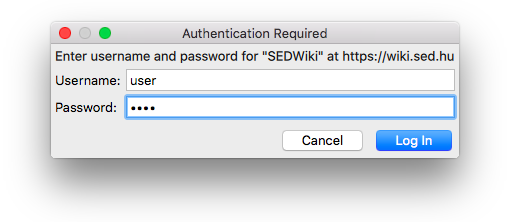
\includegraphics[scale=0.75]{ad-quick-screenshot}
    \caption{
        \label{fig:ad-quick-screenshot}
        \texttt{AuthenticationDialog} QML típus
    }
\end{figure}

A javítások és az új Quick Authentication Dialog ablak a Qt 5.6-os verziójában jelentek meg.


\section{Favicon Manager}

\noindent
A \textbf{favicon} a web oldalhoz tartozó ikon, vagy más néven \textit{shortcut icon}. A
favicon-t web oldal HTML kódjában kell megadni az alábbi módon:
\begin{verbatim}
<html>
    <head>
        <link rel="shortcut icon" href="favicon.png" />
    </head>
</html>
\end{verbatim}
A böngészőalkalmazás ezt az ikont tetszőleges célokra használhatja fel, jellemzően az URL
bar-on vagy a tab-on jelenítik meg.
Az oldalhoz rendelt ikon lehet \textit{touch icon} is. A touch icon többnyire nagyobb
felbontású, mint a favicon és elsősorban érintőképernyős készülékeken használják az
előzmények és/vagy könyvjelzők megjelenítésére. Egy oldalhoz több favicon és/vagy touch icon
is tartozhat, böngészőalkalmazás feladata választani közülük.

A Qt WebEngine-ben megvalósított \textbf{Favicon Manager} ezeket az ikonokat tölti le a
Chromium Content API-n keresztül, tárolja azokat és implementál belső API-t az elérésükre.
Megvalósítását több cél is motiválta:
\begin{itemize}
    \item Az jelszóval védett oldalak betöltése esetén ne legyen szükség workaround-ra a
        böngészőalkalmazás kódjában ahhoz, hogy le lehessen tölteni egy ikont
    \item A Qt WebEngine korábbi verziói nem támogatták a touch icon-ok használatát
    \item A Qt WebEngine korábbi verziói nem támogatták az ikonok közötti választást
    \item Bizonyos esetekben a touch icon-ok közül is a legnagyobb felbontásúra van szükség
\end{itemize}

Mivel a Favicon Manager megvalósítása sok részfeladatot foglal magában, ezért ezek
rendszerezésére egy gyűjtő issue-t készítettem:
\begin{center}
    \begin{issuebox}
        \begin{itemize}
            \renewcommand{\labelitemi}{\textcolor{qtred}{$\blacktriangleright$}}
            \item \qtbug{51179}
        \end{itemize}
    \end{issuebox}
\end{center}
Ebben a fejezetben felsorolt patch-ek egy-egy részfeladatot valósítanak meg. Egy részük
új funkciót vezetnek meg, míg mások hiba javításokat vagy teszteket tartalmaznak.

\begin{center}
    \begin{reviewbox}
        \begin{itemize}
            \renewcommand{\labelitemi}{\textcolor{qtgreen}{$\blacktriangleright$}}
            \item \gerrit{127480}
            \item \gerrit{148542}
        \end{itemize}
    \end{reviewbox}
\end{center}

Az új funkció alapját a WebEngine Core modulban implementált \texttt{FaviconManager} osztály
valósítja meg. Ez az osztály tölti le a megjelenített oldalhoz tartozó ikonokat,
választja ki közülük a megfelelőt, jelez a publikus API-nak ha a view-hoz rendelt ikon
megváltozott, a publikus API ezen keresztül tudja lekérni az ikont.
A kódban már a C++11 szabvány \textit{range-based for} nyelvi elemét használtam fel az
iterációkhoz az optimális megvalósítás érdekében.

Az ikonok letöltéséhez a Content API \texttt{WebContents::DownloadImage()} \\
függvényét használom, ezáltal nincs szükség külön implementációra az autentikációhoz, azt a
Content API elvégzi. Abban az esetben, ha az ikon QRC-ben (Qt Resource System)\footnote{A Qt
    ezen funkciójával teszi azt lehetővé, hogy a Qt-s alkalmazáshoz tartozó fájlokat a
    binárison belül tároljuk. A Chromium nem támogatja ezt a protokollt.}
van tárolva, az ikon betöltése Qt API-n keresztül történik, nincs szükség letöltésre.

A Favicon Manager a web oldalhoz tartozó összes ikont megpróbálja letölteni és azokat egy
\texttt{QMap}-ben tárolja. A map-ből az ikont az URL-je alapján lehet elérni. A Favicon
Manager letöltés előtt ellenőrzi, hogy a map-ben benne van e már az ikon, ha benne van,
nem ismétli meg a letöltést, így gyorsítótárazva (cache) az ikonokat.

Minden tabhoz (WebEngineView-hoz) saját Favicon Manager tartozik, ezért előfordulhat, egy
bizonyos ikon többször van tárolva a memóriában. Ennek a modellnek az előnye a gyorsabb
keresés és az egyszerűbb implementáció. A publikus WebEngineView API a
\texttt{iconChanged()} signal-al jelzi, hogy ha megváltozott a view-hoz tartozó ikon.
Ez az ikon a publikus API-n keresztül lekérhető (\texttt{icon} és \texttt{iconUrl}
property-k), az API pedig a Favicon Manager-től kéri el.
A Favicon Manager a letöltött ikonok közül a legnagyobb felbontásút fogja felajánlani.

A publikus API-k közvetlenül nem változtak, viszont működésük némileg igen. Így indokolttá
vált a Quick és Widget API-k favicon tesztjeinek kibővítése és lefedettségük növelése, ami
az első Favicon Manager-t megvalósító patch jelentős részét teszi ki.

\begin{center}
    \begin{reviewbox}
        \begin{itemize}
            \renewcommand{\labelitemi}{\textcolor{qtgreen}{$\blacktriangleright$}}
            \item \gerrit{150667}
            \item \gerrit{150668}
            \item \gerrit{153438}
        \end{itemize}
    \end{reviewbox}
\end{center}

A publikus Favicon Manager publikus API-jának fejlesztése során több változat is született.
Végül úgy döntöttünk, hogy az 5.7-es verzióban nem lesz a Favicon Manager-nek publikus
API-ja, hanem a már meglévő ikon API-k lesznek tovább fejlesztve. Habár a tervezett
funkcionalitások még bevezetésre kerülhetnek a Qt 5.8-as verziójában, karbantarthatóság
miatt az ezt támogató WebEngine Core-ban implementált funkciókat eltávolítottam.
A Favicon Manager implementációjának karbantartása mellett, a fejlesztés közben megtalált
hibákat is javítottam.

\begin{center}
    \begin{reviewbox}
        \begin{itemize}
            \renewcommand{\labelitemi}{\textcolor{qtgreen}{$\blacktriangleright$}}
            \item \gerrit{151057}
        \end{itemize}
    \end{reviewbox}
\end{center}

Habár új publikus API-t nem vezettünk be a Favicon Manager-hez, mindenképpen szerettem volna,
hogy ha a fejlesztőnek van kontrollja az ikonok letöltése felett. Ennek megvalósításához
a \texttt{WebEngineSettings}-hez adtam hozzá új beállításokat:
\begin{description}
    \item[\texttt{AutoLoadIconsForPage}] Az ikonok automatikusan legyenek letöltve
    \item[\texttt{TouchIconsEnabled}] Legyenek letiltva a touch ikonok is
\end{description}

A \texttt{AutoLoadIconsForPage} beállítás alapértelmezetten engedélyezve van, letiltásával
a Qt WebEngine nem tölti le az ikonokat, ezáltal a böngészőalkalmazás gyorsabb lehet,
spórolhat a sávszélességen, továbbá a fejlesztőnek van lehetősége saját ikon manager-t
implementálni úgy, hogy ne kelljen törődnie a Qt WebEngine API ikon signal-jaival.

A \texttt{TouchIconsEnabled} beállítás desktop környezetben alapértelmezetten le van tiltva.
Egy klasszikus desktop böngészőalkalmazásnak nincs szüksége touch ikonokra.

\begin{center}
    \begin{reviewbox}
        \begin{itemize}
            \renewcommand{\labelitemi}{\textcolor{qtgreen}{$\blacktriangleright$}}
            \item \gerrit{151314}
            \item \gerrit{151315}
            \item \gerrit{157142}
        \end{itemize}
    \end{reviewbox}
\end{center}

Önmagában a Favicon Manager megvalósítása a WebEngine Core modulban nem sok előnyt nyújt.
Szükséges a publikus API-k módosítása is, hogy kihasználják a Favicon Manager által nyújtott
lehetőségeket. Az API-k bővítését a Widget API-val kezdtem, mivel annak megvalósítása
egyszerűbb és a WebEngine Widgets modulra épülő demobrowser-ben a Favicon Manager haszna
jól demonstrálható.

A WebEngineWidgets module két API-t is nyújt az ikonok elérésére. Az egyik a
\texttt{QWebEnginePage}, a másik a \texttt{QWebEngineView}. A kettő lényegében ugyanaz:
a \texttt{QWebEnginePage} \texttt{iconUrl} property-jén keresztül elérhető a page-hez
tartozó ikon URL-je, amennyiben ez az URL megváltozik akkor egy \texttt{iconUrlChanged}
signal-t küld. A \texttt{QWebEngineView} ugyanezt a property-t és a hozzátartozó signal-t
valósítja meg, csak az éppen megjelenített page-hez tartozó URL-t adja vissza.

Az API-k egy új \texttt{icon} property-vel és a hozzátartozó \texttt{iconChanged} signal-al
lettek bővítve. Az új property a már meglévő \texttt{iconUrl} property-hez hasonlóan működik,
azzal az eltéréssel, hogy nem az ikon URL-jét tartalmazza, hanem az URL-ről letöltött ikont
egy \texttt{QIcon} példányban tárolva. Az új property-nek hála a böngészőalkalmazásnak nem
kell megvalósítania a letöltést, így a demobrowser példa böngészőalkalmazásból is
eltávolítottam a \texttt{QNetworkAccessManager} használatát és az autentikációhoz szükséges
workaround-ot is.

Az bővített API-val most már a WebEngine Widgets modul támogatja az olyan ikonok használatát
is, amelyek több különböző méretű ikont ágyaznak magukba (\textit{multi-size icon}).
Ezekhez, és az új \texttt{icon} property-hez teszteket is készítettem,
a \texttt{QWebEnginePage} és \texttt{QWebEngineView} API-k dokumentációit bővítettem és
naprakésszé tettem.

\begin{center}
    \begin{reviewbox}
        \begin{itemize}
            \renewcommand{\labelitemi}{\textcolor{qtgreen}{$\blacktriangleright$}}
            \item \gerrit{154018}
            \item \gerrit{156213}
        \end{itemize}
    \end{reviewbox}
\end{center}

A WebEngine QML API esetében a Widget-hez hasonló bővítés megvalósítás sokkal bonyolultabb
volt, mivel sem a QML, sem a Quick nem nyújt ikon támogatást. Az ikon megjelenítésére az
\texttt{Image} QML típus használható, viszont annak az API-ja csak URL alapján tud képet
betölteni. A Favicon Manager a letöltött ikont a memóriában tárolja és nem érhető el URL-el.

Erre a problémára megoldást a Quick API \texttt{QQuickImageProvider} interface-e nyújt
megoldást. A QML context-ben beregisztrált image provider egy speciális URL-el rendelkezik,
ha az \texttt{Image} QML típus egy ilyen URL-t kap forrásként, akkor a kérést a provider-hez
irányítja, amely betölti az \texttt{Image}-be a megfelelő képet.

Az új \texttt{QQuickWebEngineFaviconProvider} osztály ezt az osztályt valósítja meg.
Amennyiben az \texttt{Image} forrás URL-je \texttt{image://favicon/url} alakú, akkor a
kérést a \texttt{QQuickWebEngineFaviconProvider}-hez irányítja, amely elkéri a
Favicon Manager-től a \texttt{url}-hez bejegyzett ikont. A \texttt{Image} rendelkezik
egy \texttt{sourceSize} property-vel is, amelynek értékét a provider megkapja, így ezt a
multi-size ikonok támogatására használtam fel. Amennyiben az URL-ben hivatkozott ikon
multi-size és a \texttt{sourceSize} be van állítva, akkor a \texttt{sourceSize}-ban definiált
mérethez legjobban illeszkedő ikont tölti be a \texttt{QQuickWebEngineFaviconProvider}.

Az új provider használatához módosítani kellett a \texttt{WebEngineView} QML típus
\texttt{icon} property-jét. Ez a property korábban az ikon eredeti URL-jét tárolta,
az új módosítással a property-ben tárolt URL a \texttt{QQuickWebEngineFaviconProvider}
speciális URL-je, amelyen keresztül elérhető a Favicon Manager-ben tárolt ikon.

A \texttt{QQuickWebEngineFaviconProvider} tesztelése külön kihívást jelentett számomra.
Mindenképpen azt szerettem volna tesztelni, hogy a provider a \texttt{sourceSize}-nak
megfelelő ikont tölti-e be. A teszt stratégiám az volt, hogy minden tesztelni kívánt mérethez
egy szürke árnyalatos ikont készítek, és ezekből egy multi-size ikont generálok. Az egyes
szürke árnyalatos ikonok az RGB színcsatornáikban a saját méretüket kódolják. Például, a
32x32-es méretű ikonnak minden pixelének RGB értéke (32, 32, 32). Teszt betöltött ikon
egy pixelének, egyik színcsatornájának értékét vizsgálja meg, hogy megegyezik-e
a \texttt{Image} QML típus \texttt{sourceSize} property-jénék értékével.

A teszt megvalósításánál a legnagyobb problémát az okozta, hogy a \texttt{Image} QML
típus nem nyújt API-t a pixelek lekérdezésére. QML-ben erre a \texttt{Canvas} típusban
van lehetőség, amely ugyan tud képet betölteni provider-ből, viszont támogat
\texttt{sourceSize} vagy ahhoz hasonló property. Ennek a problémának a megoldására egy
sor workaround-ra volt szükség, de végül sikerült a betöltött ikon egy pixelét QML és
JavaScript kóddal lekérdezni. Ezen speciális teszt megvalósítása során sikerült a
Qt Declarative komponens Quick moduljában is hibát találni, amit ki is javítottam.

\begin{center}
    \begin{reviewbox}
        \begin{itemize}
            \renewcommand{\labelitemi}{\textcolor{qtgreen}{$\blacktriangleright$}}
            \item \gerrit{155559}
        \end{itemize}
    \end{reviewbox}
\end{center}

Mivel sikerült a Qt WebEngine Quick és Widget API-jait úgy bővíteni, hogy képesek legyenek
támogatni a multi-size ikonokat, így kompromisszumos megoldásnak tűnt külön Favicon Manager
API helyett ezt a funkciót felhasználni arra, hogy egy adott oldalhoz elérhető ikonok
(\textit{candidate icons}) listájából válogatni lehessen.

A megvalósításban a Favicon Manager a candidate ikonokat egy multi-size ikonba gyűjti össze.
Azonos méretű ikonok esetén csak az marad bent, amelyik először került bele a multi-size
ikonba. Amikor a böngészőalkalmazás lekéri az ikont a WebEngine-től akkor ezt az ikont
fogja megkapni. Az ikon méretezésének megfelelően a méretben legmegfelelőbb ikon kerül
betöltésre.

A Widget API esetében a méretezést a \texttt{QIcon} API-ján keresztül történik, míg a
Quick API esetén a \texttt{QQuickWebEngineFaviconProvider}-en keresztül a már leírtak
szerint. Ebből kifolyólag a tesztelés is hasonlóan történik, mint a multi-size ikonok
esetén.

\begin{center}
    \begin{reviewbox}
        \begin{itemize}
            \renewcommand{\labelitemi}{\textcolor{qtgreen}{$\blacktriangleright$}}
            \item \gerrit{156064}
        \end{itemize}
    \end{reviewbox}
\end{center}

Böngészőkben az ikonokkal nem csak az éppen látható oldalt azonosíthatjuk, hanem a már
látogatottakat is. A Quick API-ban korábban nem volt lehetőség a böngészési előzményekhez
rendelt ikonokhoz hozzáférni. A továbbfejlesztett Navigation History API-ban már elérhető
az előzményekhez rendelt \texttt{QQuickWebEngineFaviconProvider} specifikus URL.

A fejezetben bemutatott Favicon Manager és az ahhoz kapcsolódó API fejlesztések a Qt 5.7-es
verziójában fognak megjelenni. A Favicon Manager publikus API-jának elkészítése tervben van,
az leghamarabb a Qt 5.8-as verziójában jelenhet meg, ha úgy döntünk, hogy szükség van rá.
További terv az 5.8-as verzióba, egy ikon adatbázis megvalósítása, ami a Qt WebKit-nek is
része. Az adatbázis segítségével az ikonok lemezre menthetőek lennének és ezáltal offline
módban is hozzáférhetőek. A tervről issue is készült:
\begin{center}
    \begin{issuebox}
        \begin{itemize}
            \renewcommand{\labelitemi}{\textcolor{qtred}{$\blacktriangleright$}}
            \item \qtbug{51184}
        \end{itemize}
    \end{issuebox}
\end{center}


\chapter{Egy példa böngészőalkalmazás megvalósítása}

A \ref{chap:features}. fejezetben bemutatott új funkciók használatát egy saját
böngészőalkalmazás segítségével mutatom be ebben a fejezetben. Az alkalmazást első sorban
desktop környezetre szántam. Mivel a Qt egy cross-platform keretrendszer így a példa
böngészőalkalmazás működik a legnépszerűbb desktop operációs rendszereken: Windows, Linux,
OS X. Mindemellett elméletileg működik beágyazott környezetben is (pl.: Embedded Linux),
ahol a Qt WebEngine támogatott (Androidon már nem), viszont ez nem került kipróbálásra.

Az alkalmazást QML nyelven valósítottam meg. Minimális C++ kód is része a megvalósításnak,
amely két részből áll. Az egyik a program fő belépési pontjának megvalósítása, amely
inicializálja a Qt WebEngine OpenGL és QML környezetét, illetve betölti a QML programot:
\begin{lstlisting}[title=main.cpp]
 int main(int argc, char *argv[])
 {
    QApplication app(argc, argv);

    QtWebEngine::initialize();

    QQmlApplicationEngine engine;
    Utils utils;
    engine.rootContext()->setContextProperty("utils", &utils);
    engine.load(QUrl(QStringLiteral("qrc:/main.qml")));

    return app.exec();
 }
\end{lstlisting}
A másik rész segédfüggvényeket implementál a QML nyelvhez, amelyek a \texttt{utils} \\
property-n elérhetőek QML-ből. A segédfüggvények az alábbiak:
\begin{description}
    \item[\texttt{fromUserInput(userInput)}] A paraméterül kapott stringet URL-é alakítja
        annak megfelelően, hogy a hivatkozott erőforrás lokálisan vagy HTTP protokollon
        keresztül érhető el
    \item[\texttt{setLocale(locale)}] A Qt alapértelmezett nyelvi beállításait definiálja
        felül a \texttt{locale} paraméterrel
\end{description}

\section{Felhasználói felület (GUI)}

A QML kód túlnyomó része a GUI-t valósítja meg. Mivel a QML egy deklaratív nyelv,
nem kellett túl sokat dolgozni a működés megvalósításán, azt a Qt WebEngine \\
Quick/QML API-ja már megvalósította. A hangsúly a megjelenés megtervezésén van,
ezért könnyű a QML nyelven programozni, a fejlesztőnek csak a GUI elemek testre szabására
és az azok közötti interakciókra kell figyelni. Lényegében a \texttt{WebEngineView} QML
típus is egy GUI elem, ami a web oldal tartalmát rajzolja egy téglalap alakú felületre és
küld értesítést (signal-okat) a nézetben történt változásokról.

A GUI megtervezésénél legfőbb szempontnak tartottam, hogy a böngészőalkalmazás desktop-ra
készül, ahol a megjelenítő szélessége nagyobb, mint a magassága. Ezzel szemben a web oldalak
általában magasabbak, mint szélesek, ezért a bal szélen ki nem használt területet a tabok
és a böngészési előzmények megjelenítésére használtam fel. A másik fontos szempont az volt,
hogy az alkalmazás ablakának minél nagyobb részét a böngészési felület
(\texttt{WebEngineView}) töltse ki. Ezt elsősorban animált, nyitható-csukható panelek
megvalósításával próbáltam elérni.

A böngészőalkalmazás megjelenését igyekeztem minél egyedibbé tenni, ezért a QML megvalósítás
több új, saját QML típust is tartalmaz. Ezek az új típusok (GUI elemek), ahol csak lehet
kihasználják a Quick keretrendszer által nyújtotta előnyöket: az elemek tulajdonságai
(méret, pozíció, szín, stb) dinamikusan változnak, az átmenetek animálva vannak, hogy
egy valódi "fluid" felületté álljanak össze.

\subsection{Vezérlők (controls)}
A legalapvetőbb ilyen elemek, amelyek valamilyen felhasználói interakcióra (első sorban
bal gombbal kattintásra) adnak választ. Ilyen vezérlő elemeket Qt QuickControls modulja
is tartalmaz, melyeket sok helyen fel is használtam. Néhány elemet azonban magam valósítottam
meg, hogy jobban illeszkedjenek a tervezett GUI-ba.

\subsubsection{Gombok}
Háromféle különböző gombot használtam fel, amelyek egy közös őstől származnak,
a saját \texttt{Button} QML típusból. A gombok működésben nem térnek el egymástól csak a
színezésük más. Egy gombnak négy állapota lehet:
\begin{description}
    \item[\texttt{released}] Alapállapot
    \item[\texttt{disabled}] A gomb le van tiltva, nem reagál felhasználói interakcióra
    \item[\texttt{hovered}] Az egérmutató a gomb felett van
    \item[\texttt{pressed}] Bal egérgombot lenyomva tartjuk a gomb felett
\end{description}

A \ref{fig:browser-button}, \ref{fig:settings-button} és \ref{fig:close-button} ábrák
mutatják be a felhasznált gombokat, rendre azok lehetséges állapotaikkal együtt.

\begin{figure}[H]
    \centering
    
\includegraphics[scale=0.8]{BrowserButton}
    \caption{
        \label{fig:browser-button}
        \texttt{BrowserButton} 4 állapota: \textit{released}, \textit{disabled},
        \textit{hovered} és \textit{pressed}
    }
\end{figure}
\begin{figure}[H]
    \centering
    
\includegraphics[scale=0.8]{SettingsButton}
    \caption{
        \label{fig:settings-button}
        \texttt{SettingsButton} 4 állapota: \textit{released}, \textit{disabled},
        \textit{hovered} és \textit{pressed}
    }
\end{figure}
\begin{figure}[H]
    \centering
    
\includegraphics[scale=0.8]{CloseButton}
    \caption{
        \label{fig:close-button}
        \texttt{CloseButton} 4 állapota: \textit{released}, \textit{disabled},
        \textit{hovered} és \textit{pressed}
    }
\end{figure}


\subsubsection{Kapcsoló}
A \texttt{BrowserSwitch} QML típus egy két állapotú kapcsolót valósít meg. Csak egy helyen
van felhasználva, viszont általánosan van megvalósítva, hogy újra felhasználható legyen.

\begin{figure}[H]
    \centering
    %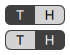
\includegraphics[scale=0.8]{BrowserSwitch-compact}
    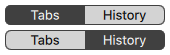
\includegraphics[scale=0.8]{BrowserSwitch-wide}
    \caption{
        \label{fig:browser-switch}
        \texttt{BrowserSwitch} 2 állapota: fent bal oldal, lent jobb oldal van kiválasztva
    }
\end{figure}

\subsubsection{Lista elem sablonok}
\label{sec:list-entry-templates}
A tabok és a böngészési előzmények listáját a \texttt{ListView} QML típus valósítja mag.
A \texttt{ListView} típus az elemeket egy sablon QML típus példányosításával
jeleníti meg. Ilyen saját template típusok a \texttt{CompactEntry} és a \texttt{WideEntry}.
\begin{figure}[H]
    \centering
    
\includegraphics[scale=0.8]{Compact-Wide-Entries}
    \caption{
        \label{fig:compact-wide-entries}
        \texttt{CompactEntry} felül és \texttt{WideEntry} alul
    }
\end{figure}
A \texttt{CompactEntry} csak a weboldal ikonját jeleníti meg nagy méretben (touch ikont, ha
van elérhető). A \texttt{WideEntry} szélessége miatt nagyobb helyet foglal, megjeleníti az
oldal kis méretű favicon-ját, mellette pedig a web oldal címét. Ezek a lista elem sablonok
tulajdonképpen nem ``vezérlők'', mert a felhasználói eseményeket nem az elem, hanem a
\texttt{ListView} QML típus kezeli le, viszont a felhasználó a lista elemre kattintva
``vezérli'' az alkalmazást.

\subsection{Nézetek (views)}
Ebbe a kategóriába olyan saját QML típusokat sorolok, amelyek más GUI elemeket fognak össze
és jelenítenek meg a nézet típusa szerint.

\subsubsection{Lista nézetek}
A \ref{sec:list-entry-templates} alfejezetben már volt arról szó, hogy a példa
böngészőalkalmazás saját sablonokat használ lista elemek létrehozására. A listák
megjelenítésére a \texttt{ListView} QML típus saját, specializált változatait használja:
\texttt{TabListView}-t a tabokhoz és \\
\texttt{HistoryListView}-t a böngészési előzményekhez.
\begin{figure}[H]
    \centering
    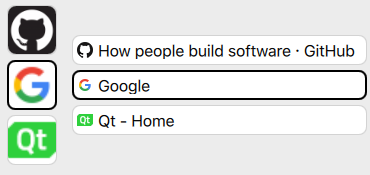
\includegraphics[scale=0.5]{TabListView}
    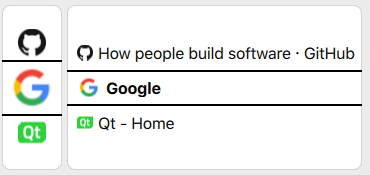
\includegraphics[scale=0.5]{HistoryListView}
    \caption{
        \label{fig:tab-list-view}
        \texttt{TabListView} és \texttt{HistoryListView}
    }
\end{figure}

\subsubsection{SliderPanel}
A \texttt{SliderPanel} egy olyan felület, amivel a GUI nem gyakran használt elemeit rejthetjük
el, vagy kicsinyítjük le a nagyobb helykihasználás érdekében. A lista nézetek esetén a
\textit{Wide} és \textit{Compact} mód közötti váltás is \texttt{SliderPanel} segítségével
történik. Ez a QML típus testre szabható, hogy vízszintesen vagy függőlegesen jelenjen meg,
illetve, hogy teljesen vagy csak részben csukódjon össze.
\begin{figure}[H]
    \centering
    
\includegraphics[scale=0.8]{SliderPanel}
    \caption{
        \label{fig:slider-panel}
        \texttt{SliderPanel} zárt és nyitott állapotban
    }
\end{figure}

\subsubsection{SettingsPanel}
A \texttt{SettingsPanel} egy dialógus ablakot megvalósító saját QML típus. A panel
mozgatható (\textit{drag}), a bezárás és az Ok gombok (\texttt{SettingsButton}) a típus
részei, beépített \textit{confirm dialog}-gal rendelkezik, a vezérlő elemek bővíthetőek
és a tartalom görgethető. A \texttt{SettingsPanel} saját stílus definíciókat is tartalmaz
a \texttt{Checkbox} és \texttt{TextField} QML típusokhoz.

\begin{figure}[H]
    \centering
    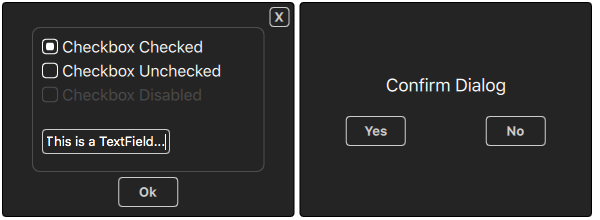
\includegraphics[scale=0.7]{SettingsPanel}
    \caption{
        \label{fig:settings-panel}
        \texttt{SettingsPanel} beállításokkal és a beépített confirm dialog-gal
    }
\end{figure}

\subsection{Qt WebEngine specifikus QML típusok}
Az alábbi típusok a nézetekhez hasonlóak, de nem általánosan újra felhasználhatóak.
Tartalmuk rögzített, melyek felhasználják a \texttt{WebEngineView} QML típus valamely \\
property-jét.

Az \texttt{AddressBar} típus a betölteni kívánt weboldal URL-jének megadására használatos.
Ez a GUI eleme interaktív, mutatja az oldal betöltésének állapotát és az oldal favicon-ját
teljesen betöltött oldal esetén.
\begin{figure}[H]
    \centering
    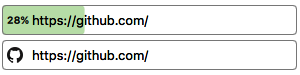
\includegraphics[scale=0.8]{AddressBar}
    \caption{
        \label{fig:address-bar}
        \texttt{AddressBar} oldal betöltés közben és betöltött oldallal
    }
\end{figure}

A \texttt{FindBar} típus kifejezetten a Qt WebEngine Find Text funkciójának használatára
lett létrehozva. Tartalmaz egy szövegmezőt a keresendő szöveg beviteléhez, gombokat
(\texttt{BrowserButton}) a találatok navigációjához és egy bezáró gombot
(\texttt{CloseButton}) a keresés alapállapotba állításához és a \texttt{FindBar}
elrejtéséhez.
\begin{figure}[H]
    \centering
    
\includegraphics[scale=0.8]{FindBar}
    \caption{
        \label{fig:find-bar}
        \texttt{FindBar}
    }
\end{figure}

\subsection{Modellek (models)}
A példa böngészőalkalmazáshoz megvalósított saját modellek valójában nem GUI része, mert
nem megjelenést definiálnak. Dinamikus tartalmat határoznak meg, amelyet más QML típusoknak
kell megjeleníteniük. A megvalósítások a \texttt{ListModel} QML típust specializálják úgy,
hogy tartalmuk egyedi módon változtatható legyen.

\subsubsection{WebEngineViewListModel}
Ez a modell az alkalmazás egyik legfontosabb eleme. Új \texttt{WebEngineView} példányok
ezen keresztül hozhatóak létre, szúrhatóak be listába, távolíthatóak el a már nem
szükséges példányok. A \texttt{TabListView} saját QML típus ennek a modellnek az elemeit
jeleníti meg.

\subsubsection{LocaleListModel}
A \texttt{LocaleListModel} tartalmazza a böngészőalkalmazás által beállítható nyelvek
listáját. Néhány nyelv a modellben előre meg van adva, példányosításkor a listába
kerül a futtató rendszer alapértelmezett nyelve is. Ezt a modellt a
\texttt{SettingsPanel}-en található, nyelv kiválasztó \texttt{ComboBox} QML típus használja.

\subsection{Összkép}
A saját és a Qt gyári QML típusai a \texttt{main.qml} QML fájlban vannak példányosítva és
összekötve. Ez az alkalmazás QML megvalósításának fő belépési pontja, amely egy \\
\texttt{ApplicationWindow} QML típusban helyezi el a GUI elemeket.

\begin{figure}[H]
    \centering
    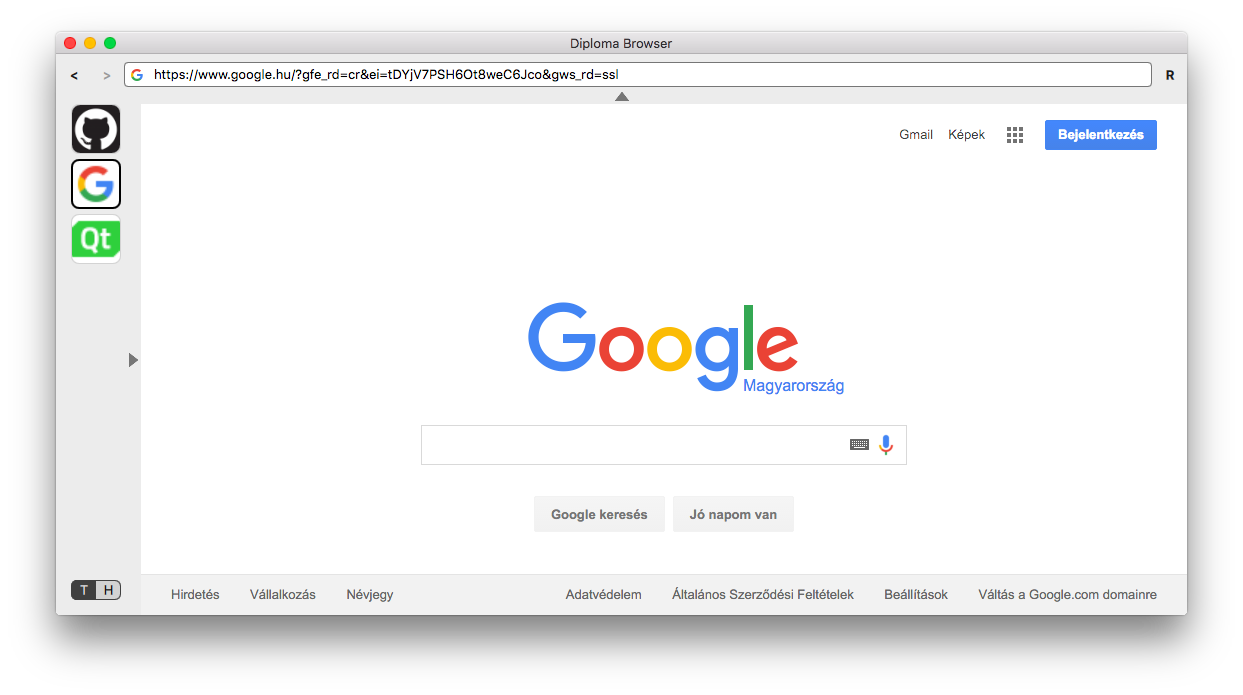
\includegraphics[scale=0.34]{diplomabrowser}
    \caption{
        \label{fig:diplomabrowser}
        A példa böngészőalkalmazás képernyőképe
    }
\end{figure}

\newpage
\section{Új Qt WebEngine funkciók használata}

Az funkciók használatának bemutatására a példa böngészőalkalmazás QML kódját használom fel.
A legtöbb esetben a példakód nem egy-egy az egyben lett bemásolva, hogy az olvashatóbb
legyen és nyomtatásban kiférjen. Minden kódrészletnél megjelöltem, hogy az eredeti
melyik forrásfájlban található. Eltávolításra kerültek még a funkcióhoz nem kapcsolódó
kódrészletek is, hogy azok ne legyenek zavaróak vagy félrevezetőek a magyarázatban.

\subsection{Favicon Manager}

A példa alkalmazásban az ikonokat minden esetben a \texttt{Image} QML típussal jelenítem meg.
Ikonok összesen három saját QML típusban fordulnak elő: \texttt{AddressBar}, \\
\texttt{CompactEntry} és \texttt{WideEntry}. Az API használata lényegében nem tér el a három
típusban, ezért azt az \texttt{AddressBar} kódjával szemléltetem:
\begin{lstlisting}[title=AddressBar.qml]
 Image {
    id: icon

    width: 16; height: 16
    sourceSize: Qt.size(width, height)
    source: root.iconUrl
    /* ... */
 }
\end{lstlisting}
A Favicon Manager szempontjából két property fontos: a \texttt{sourceSize} és a
\texttt{source}. A \texttt{sourceSize} property mondja meg, hogy mekkora ikont kell
betöltenie a Favicon Provider-nek. Jelen esetben ez úgy van megadva, hogy egyezzen meg az
\texttt{Image} elem méretével, így az ha dinamikusan változik, akkor a Favicon Provider
implicit az új méretnek megfelelő ikont tölti be.

A \texttt{source} property értékének egy, a Favicon Provider-re hivatkozó URL-nek kell lennie.
Ezt az URL-t a \texttt{WebEngineView::icon} property tárolja. Azért, hogy az \\
\texttt{AddressBar} típusnak ne kelljen beimportálnia a Qt WebEngine modult, ezért a saját
\texttt{iconUrl} property-jén keresztül éri el az URL-t. Az \texttt{iconUrl} property-nek az \\
\texttt{AddressBar} létrehozásakor kell értéket adni:
\begin{lstlisting}[title=main.qml]
 AddressBar {
    id: addressBar

    iconUrl: currentWebEngineView
                ? currentWebEngineView.icon
                : ""
    /* ... */
 }
\end{lstlisting}
Az ellenőrzésre azért van szükség, hogy az alkalmazás ne küldjön hiba üzenetet, ha nincs
megnyitva tab. Ha a \texttt{WebEngineView} példány \texttt{icon} property-je megváltozik
(új ikon töltődik be), akkor az \texttt{AddressBar} \texttt{iconUrl} property-je is
automatikusan változni fog. Ez a QML nyelv \textit{property binding} támogatása miatt
lehetséges, így a példa alkalmazásban nincs is szükség a \texttt{iconChanged} signal
használatára.

A Favicon Manager megvalósításának része, hogy a publikus \\
\texttt{WebEngineSettings}
API-n keresztül befolyásolni lehessen az ikonok letöltését. Erre kétféleképpen lehetünk
hatással: letilthatjuk az ikonok automatikus letöltését és engedélyezhetjük a touch
ikonok letöltését\footnote{Alapértelmezetten a favicon-okat automatikusan letöltjük a touch
ikonokat nem}. A beállítások tartós tárolására \texttt{Settings} QML típust használtam fel:
\begin{lstlisting}[title=main.qml]
 Settings {
    id: appSettings

    property alias autoLoadIconsForPage:
                                    autoLoadIconsForPage.checked
    property alias touchIconsEnabled: touchIconsEnabled.checked
    /* ... */
 }
\end{lstlisting}
A \texttt{Settings}-ben a \texttt{autoLoadIconsForPage} és \texttt{touchIconsEnabled}
azonosítójú \texttt{Checkbox}-ok állapotát tárolom. A \texttt{WebEngineSettings} megfelelő
property-jeit ezek szerint a beállítások szerint inicializálom, amikor létre jön egy új \\
\texttt{WebEngineView}:
\begin{lstlisting}[title=main.qml]
 WebEngineViewListModel {
    id: viewListModel

    onCreated: {
        webEngineView.settings.autoLoadIconsForPage =
            Qt.binding(function() {
                return appSettings.autoLoadIconsForPage;
            });
        webEngineView.settings.touchIconsEnabled =
            Qt.binding(function() {
                return appSettings.touchIconsEnabled;
            });
        /* ... */
    }

    /* ... */
 }
\end{lstlisting}
Ezzel a megoldással a böngésző alkalmazás a legutóbbi kilépéskori beállításokkal indul. A
\texttt{Qt.binding()} JavaScript függvény hívásra azért van szükség, hogy kikényszerítsem
a \texttt{QML} property binding-ot: amikor a checkbox-ok állapota változik és azzal együtt
a \texttt{appSetttings}-é is, úgy automatikusan változnak a \texttt{WebEngineSettings}
bekötött property-jei is.


\subsection{Navigation History}

\noindent
\textbf{main.qml:}
\begin{verbatim}
HistoryListView {
    id: historyListView
    model: currentWebEngineView ?
            currentWebEngineView.navigationHistory.items :
            undefined

    onSelected: {
        navigationAnimation.start();
        currentWebEngineView.goBackOrForward(offset);
    }

    /* ... */
}
\end{verbatim}

\noindent
\textbf{views/HistoryListView.qml:}
\begin{verbatim}
property Component compactDelegate: Component {
    CompactEntry {
        iconUrl: icon ? icon : ""

        /* ... */

        onClicked: {
            if (currentIndex == index)
                return;
            root.currentIndex = index;
            root.selected(offset);
        }
    }
}

property Component wideDelegate : Component {
    WideEntry {
        iconUrl: icon ? icon : ""
        pageTitle: title ? title : ""

        /* ... */

        onClicked: {
            if (currentIndex == index)
                return;
            root.currentIndex = index;
            root.selected(offset);
        }
    }
}
\end{verbatim}

\begin{itemize}
    \item \texttt{navigationHistory} property hol van használva?
        \begin{itemize}
            \item \texttt{HistoryListView}
        \end{itemize}
    \item role-ok hol, hogyan vannak használva: lista elem sablonok
        \begin{itemize}
            \item \texttt{title} role
            \item \texttt{offset} role
            \item \texttt{icon} role
        \end{itemize}
\end{itemize}

\subsection{Find Text}

\noindent
\textbf{main.qml:}
\begin{verbatim}
FindBar {
    id: findBar

    onFindNext: currentWebEngineView.findText(text)
    onFindPrev: currentWebEngineView.findText(text,
                            WebEngineView.FindBackward)

    onStateChanged: {
        if (state == "hidden" && currentWebEngineView) {
            currentWebEngineView.findText("");
            currentWebEngineView.forceActiveFocus();
        }
    }
}
\end{verbatim}

\subsection{Form Validation és Localization}

\noindent
\textbf{main.qml:}
\begin{verbatim}
ComboBox {
    id: localeCombo

    model: LocaleListModel { }
    textRole: "name"

    property string locale: appSettings.locale
    onCountChanged: currentIndex = model.findLocale(locale)
    onCurrentIndexChanged: localeCombo.locale =
                            model.get(currentIndex).locale
}
\end{verbatim}

\noindent
\textbf{main.qml:}
\begin{verbatim}
SettingsPanel {
    id: settingsPanel

    property string locale: appSettings.locale

    onAccepted: {
        homeUrl = utils.fromUserInput(homeUrlField.text);
        if (locale != localeCombo.locale) {
            locale = localeCombo.locale;
            utils.setLocale(locale);
            settingsPanel.state = "confirm";
        } else
            settingsPanel.state = "hidden";
    }

    onRestartRequest: {
        for (var i = 0; i < viewListModel.count; ++i)
            viewListModel.restart(i);
    }

    /* ... */
}
\end{verbatim}

\begin{figure}[H]
    \centering
    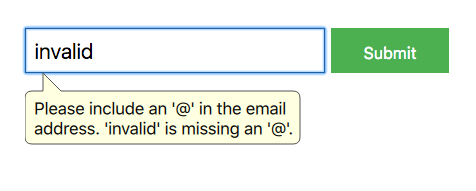
\includegraphics[scale=0.44]{validation-message-english}
    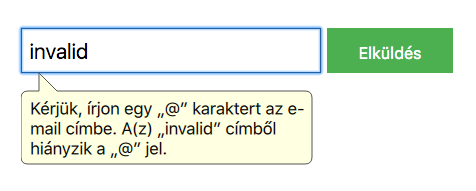
\includegraphics[scale=0.44]{validation-message-magyar}
    \caption{
        \label{fig:validation-message-localization}
        Form Validation angolul és magyarul
    }
\end{figure}


\addtocontents{toc}{\ }
\chapter*{Eredmények}
\addcontentsline{toc}{section}{Eredmények}
\begin{itemize}
    \item Eredmények:
        \begin{itemize}
            \item Hány darab új feature? Milyen kategória (QtWebKit, Test/Debug, HTML5)?
            \item Teszt lefedettség?
            \item Hány db patch ment be? Melyik milyen jellegű?
                \begin{itemize}
                    \item Új feature
                    \item Új teszt
                    \item Bug fix, build fix, teszt javítás
                    \item Chromium fork karbantartás
                    \item \dots
                \end{itemize}
            \item Chromium fork külön repository, oda is mentek patch-ek
            \item Javításaim között vannak olyanok, amelyek kimondottan platform specifikus
                problémát javítanak. Ezek lefedik a 3 fő desktop platformot: GNU/Linux,
                Windows, OS X
        \end{itemize}
    \item Összegzés?
        \begin{itemize}
            \item Hol tartunk most a QtWebKit leváltással? Mi hiányzik még?
            \item Jelenleg Qt 5.7-en dolgozunk, a felsorolásból mely feature-ök kerülnek
                be az 5.7-be: \textbf{favicon}
            \item Jövő: milyen tervek vannak 5.8-ra?
        \end{itemize}
\end{itemize}


%%% EPILOGUE %%%

\begin{thebibliography}{9}
    \addcontentsline{toc}{section}{Irodalomjegyzék}

    \bibitem{bib:qt-blog-introducing-qtwebengine}
        Qt Blog: Introducing the Qt WebEngine \\
        \href{http://blog.qt.io/blog/2013/09/12/introducing-the-qt-webengine/}
        {http://blog.qt.io/blog/2013/09/12/\\
        introducing-the-qt-webengine/}

    \bibitem{bib:wiki-chromium}
        Wikipedia: Chromium (web browser) \\
        \url{https://en.wikipedia.org/wiki/Chromium_(web_browser)}

    \bibitem{bib:wiki-chrome}
        Wikipedia: Google Chrome \\
        \url{https://en.wikipedia.org/wiki/Google_Chrome}

    \bibitem{bib:wiki-blink}
        Wikipedia: Blink (web engine) \\
        \url{https://en.wikipedia.org/wiki/Blink_(web_engine)}

    \bibitem{bib:chromium-displays-web-pages}
        Chromium: How Chromium Displays Web Pages \\
        \href{https://www.chromium.org/developers/design-documents/displaying-a-web-page-in-chrome}
        {https://www.chromium.org/developers/design-documents/\\
         displaying-a-web-page-in-chrome}

    \bibitem{bib:chromium-blink}
        Chromium: Blink \\
        \url{http://www.chromium.org/blink}

    \bibitem{bib:chromium-gpu}
        Chromium: GPU Accelerated Compositing in Chrome \\
        \href{https://www.chromium.org/developers/design-documents/gpu-accelerated-compositing-in-chrome}
        {https://www.chromium.org/developers/design-documents/\\
        gpu-accelerated-compositing-in-chrome}

    \bibitem{bib:chromium-oopifs}
        Chromium: Rendering and compositing out of process iframes \\
        \href{https://www.chromium.org/developers/design-documents/oop-iframes/oop-iframes-rendering}
        {https://www.chromium.org/developers/design-documents/\\
        oop-iframes/oop-iframes-rendering}

    \bibitem{bib:chromium-texture-mailbox}
        Chromium: CHROMIUM\_texture\_mailbox.txt \\
        \href{https://src.chromium.org/viewvc/chrome/trunk/src/gpu/GLES2/extensions/CHROMIUM/CHROMIUM_texture_mailbox.txt}
        {https://src.chromium.org/viewvc/chrome/trunk/src/gpu/\\
        GLES2/extensions/CHROMIUM/CHROMIUM\_texture\_mailbox.txt}

    \bibitem{bib:webkit-webkit2}
        WebKit: WebKit2 \\
        \url{https://trac.webkit.org/wiki/WebKit2}

    \bibitem{bib:chromium-multi-process}
        Chromium: Multi-process Architecture \\
        \href{https://www.chromium.org/developers/design-documents/multi-process-architecture}
        {https://www.chromium.org/developers/design-documents/\\
        multi-process-architecture}

    \bibitem{bib:chromium-blog-multi-process}
        Chromium Blog: Multi-process Architecture \\
        \href{http://blog.chromium.org/2008/09/multi-process-architecture.html}
        {http://blog.chromium.org/2008/09/\\
        multi-process-architecture.html}

    \bibitem{bib:chromium-process-models}
        Chromium: Process Models \\
        \href{https://www.chromium.org/developers/design-documents/process-models}
        {https://www.chromium.org/developers/design-documents/\\
        process-models}

    \bibitem{bib:chromium-plugins}
        Chromium: Plugin Architecture \\
        \href{https://www.chromium.org/developers/design-documents/plugin-architecture}
        {https://www.chromium.org/developers/design-documents/\\
        plugin-architecture}

    \bibitem{bib:chromium-content-module}
        Chromium: Content module \\
        \url{https://www.chromium.org/developers/content-module}

    \bibitem{bib:chromium-content-api}
        Chromium: Content API \\
        \href{https://www.chromium.org/developers/content-module/content-api}
        {https://www.chromium.org/developers/content-module/\\
        content-api}

    \bibitem{bib:qt-wiki-about-qt}
        Qt Wiki: About Qt \\
        \url{https://wiki.qt.io/About_Qt}

    \bibitem{bib:qt-wiki-qt-history}
        Qt Wiki: Qt History \\
        \url{https://wiki.qt.io/Qt_History}

    \bibitem{bib:qt-doc-webengine-overview}
        Qt Documentation: Qt WebEngine Overview \\
        \url{http://doc.qt.io/qt-5/qtwebengine-overview.html}

    \bibitem{bib:qt-about-us}
        The Qt Company: About Us \\
        \url{http://www.qt.io/about-us}

    \bibitem{bib:qt-doc-qtmodules}
        Qt Documentation: All Modules \\
        \url{http://doc.qt.io/qt-5/qtmodules.html}

    \bibitem{bib:qt-doc-qt-gui}
        Qt Documentation: Qt GUI \\
        \url{http://doc.qt.io/qt-5/qtgui-index.html}

    \bibitem{bib:qt-doc-user-interfaces}
        Qt Documentation: User Interfaces \\
        \url{http://doc.qt.io/qt-5/topics-ui.html}

    \bibitem{bib:qt-doc-qt-widgets}
        Qt Documentation: Qt Widgets \\
        \url{http://doc.qt.io/qt-5/qtwidgets-index.html}

    \bibitem{bib:qt-doc-qt-qml}
        Qt Documentation: Qt QML \\
        \url{http://doc.qt.io/qt-5/qtqml-index.html}

    \bibitem{bib:qt-doc-qt-quick}
        Qt Documentation: Qt Quick \\
        \url{http://doc.qt.io/qt-5/qtquick-index.html}

    \bibitem{bib:qt-doc-qt-quick-scene-graph}
        Qt Documentation: Qt Quick Scene Graph \\
        \href{http://doc.qt.io/qt-5/qtquick-visualcanvas-scenegraph.html}
        {http://doc.qt.io/qt-5/\\
        qtquick-visualcanvas-scenegraph.html}

    \bibitem{bib:qt-doc-qt-webview}
        Qt Documentation: Qt WebView \\
        \url{http://doc.qt.io/qt-5/qtwebview-index.html}

    \bibitem{bib:qt-doc-qt-websockets}
        Qt Documentation: Qt WebSockets \\
        \url{http://doc.qt.io/qt-5/qtwebsockets-index.html}

    \bibitem{bib:qt-doc-qt-webchannel}
        Qt Documentation: Qt WebChannel \\
        \url{http://doc.qt.io/qt-5/qtwebchannel-index.html}

    \bibitem{bib:kdab-qt-webchannel}
        KDAB: Qt WebChannel: bridging the gap between C++/QML and the web \\
        \url{http://doc.qt.io/qt-5/qtwebchannel-index.html}

    \bibitem{bib:qt-wiki-d-pointer}
        Qt Wiki: D-Pointer \\
        \url{https://wiki.qt.io/D-Pointer}

\end{thebibliography}


\chapter*{Nyilatkozat}
\addcontentsline{toc}{section}{Nyilatkozat}

\noindent
Alulírott Varga Péter programtervező informatikus MSc szakos hallgató, kijelentem, hogy a
dolgozatomat a Szegedi Tudományegyetem, Informatikai Tanszékcsoport Szoftverfejlesztés
Tanszékén készítettem, programtervező informatikus MSc diploma megszerzése érdekében.

Kijelentem, hogy a dolgozatot más szakon korábban nem védtem meg, saját munkám eredménye
és csak hivatkozott forrásokat (szakirodalom eszközök, stb.) használtam fel.

Tudomásul veszem, hogy a diplomamunkámat a Szegedi Tudományegyetem Informatikai Tanszékcsoport
könyvtárában, a helyben olvasható könyvek között helyezik el.

\vspace*{2cm}

\begin{tabular}{lc}
    Szeged, \today \hspace{2cm} & \makebox[6cm]{\dotfill} \\
                                & aláírás
\end{tabular}


\chapter*{Köszönetnyílvánítás}
\addcontentsline{toc}{section}{Köszönetnyílvánítás}

\noindent
Szeretnék köszönetet mondani Dr. Kiss Ákos témavezetőmnek a téma kutatása alatt nyújtott
támogatásáért és a diplomamunkám megírásában nyújtott segítségéért.

Ezen kívül szeretnék köszönetet mondani a \textit{The Qt Company} és a
\textit{Szegedi Tudományegyetem Szoftverfejlesztés Tanszék} volt es jelenleg is a QtWebEngine
projekten dolgozó munkatársainak a beszélgetésekért és a közösségnek benyújtott munkám
ellenőrzéséért és befogadásáért.


\chapter*{Mellékletek}
\addcontentsline{toc}{section}{Mellékletek}

\noindent
DVD lemez mely tartalmazza:
\begin{itemize}
    \item \texttt{QtWebEngine} modul \texttt{Git} repository-ját
    \item A bemutatott funkciókat megvalósító patch-eket
    \item A példa böngészőalkalmazás forráskódját
\end{itemize}

\end{document}
